\documentclass[12pt]{article}
\usepackage[utf8]{inputenc}
\usepackage[T1]{fontenc}
\usepackage{amsmath}
\usepackage{amsfonts}
\usepackage{amssymb}
\usepackage[version=4]{mhchem}
\usepackage{stmaryrd}
\usepackage{bbold}
\usepackage{graphicx}
\usepackage[export]{adjustbox}
\graphicspath{ {./images/} }

\usepackage{listings} % Required for insertion of code
\usepackage{xcolor} % Required for custom colors

% Define custom colors
\definecolor{codegreen}{rgb}{0,0.6,0}
\definecolor{codegray}{rgb}{0.5,0.5,0.5}
\definecolor{codepurple}{rgb}{0.58,0,0.82}
\definecolor{backcolour}{rgb}{0.95,0.95,0.92}

% Setup the style for code listings
\lstdefinestyle{mystyle}{
    backgroundcolor=\color{backcolour},   
    commentstyle=\color{codegreen},
    keywordstyle=\color{magenta},
    numberstyle=\tiny\color{codegray},
    stringstyle=\color{codepurple},
    basicstyle=\ttfamily\footnotesize,
    breakatwhitespace=false,         
    breaklines=true,                 
    captionpos=b,                    
    keepspaces=true,                 
    numbers=left,                    
    numbersep=5pt,                  
    showspaces=false,                
    showstringspaces=false,
    showtabs=false,                  
    tabsize=2
}

% Activate the style
\lstset{style=mystyle}

\title{Assignment 2: Entanglement entropy and compression of quantum states }


\author{Instructor: Lesik Motrunich\\
TA: Liam O'Brien}
\date{}


\begin{document}
\maketitle
Ph 121C: Computational Physics Lab, Spring 2024

California Institute of Technology

Due: 4pm Tuesday, April 30, 2024

\section*{1 Introduction to many-body entanglement}
In this assignment we will study a property of quantum many-body states called entanglement. It may not seem as directly physically motivated as the measures we encountered in the previous assignment, like decay of correlations or measurements of the order parameter, but it turns out that a great deal of the physics of a quantum system is closely related to its entanglement structure. In particular, one quantity called the entanglement entropy is a crucial indicator of a system's low-energy behavior, in addition to determining the degree of difficulty of simulating it on classical architecture like your computer. That the same quantity is important in both situations is not coincidental: in fact, it is typically the case that at low energies nature - that is, physically-motivated Hamiltonians - tends to favor precisely those quantum states which are more amenable to classical simulation. This fortunate state of affairs is rigorously described by the "area law," an upper bound on entanglement (proved in one dimension) which has attracted much recent interest from the quantum information and condensed matter physics communities. This principle is fundamental to our efforts in this course to overcome the limitations of exact diagonalization.

We will learn how to exploit nature's tendency to favor "simple" quantum wavefunctions by developing a compression scheme based on our physical understanding. The most evident advantage here is storage: recall that a generic eigenstate of a quantum system of even moderate size quickly becomes too big to save on a computer. What simplifications can be made to reduce the exponential scaling of the number of coefficients, while still leaving the interesting properties of a state intact? This question is nontrivial: for example, if you have an ED wavefunction from the previous assignment saved to disk as binary file you will likely find it cannot be compressed very much by tar or other generic tools, and moreover the quantum state would be opaque to us in this form. We will instead make use of the entanglement structure of the physical system to write an ansatz for one-dimensional quantum ground states called matrix product states (MPS). This ansatz is of paramount importance to a modern understanding of quantum systems in one dimension and has a strong physical motivation in the connection between entanglement and locality.

\section*{2 Singular value decomposition}
\subsection*{2.1 Matrix approximation}
Suppose you have a large collection of $m$ data points of some type, each containing a measurement of a large number $n$ of attributes. In order to study the data, one can think of each data point as a vector in an $n$-dimensional space, where each attribute is assigned to a basis vector. Then the measured value of data point $x_{i}, i \in\{1, \ldots, m\}$, for attribute $\hat{e}_{j}, j \in\{1, \ldots, n\}$, is the $j$-th entry in the vector $x_{i}$, viewed as a row vector. It is interesting, both practically and in order to understand the processes behind the data, to ask whether the points (with average subtracted) display clustering in certain directions, described by linear relationships between the basis states. If so, the subspace spanned by the dominant directions can provide a good low-dimensional projection of the data despite having reduced dimension. This is the goal of "principal component analysis," (PCA) in which one uses a low-dimensional ellipsoid to approximate data. While we are not specifically interested in PCA, it is similar to the wavefunction compression we study in spirit and some technical details; however in our case the low-dimensional representation can be exact.

To determine such principal vectors, combine the data points into an $m \times n$ data matrix $M$ of rank $r \leq \min (m, n)$. Determining a subspace of dimension $k<r$ which optimally describes the data then corresponds to finding a rank- $k$ matrix $\tilde{M}$ which minimizes the distance $\|\tilde{M}-M\|_{F}$. (Here $\|A\|_{F}=\sqrt{\operatorname{tr}\left(A^{\dagger} A\right)}$ is the so-called Frobenius norm of matrix $A$.) This is accomplished through a general method of matrix factorization known as the singular value decomposition (SVD):


\begin{equation*}
M=U S V^{\dagger} ; \quad U^{\dagger} U=V^{\dagger} V=\mathbb{I}, \quad S \text { diagonal. } \tag{1}
\end{equation*}


The SVD can be thought of as a generalization of the spectral theorem to nonsquare matrices, where the left singular vectors $\boldsymbol{u}_{\alpha}, \alpha=\{1, \ldots, r\}$, stored in $U=\left[\begin{array}{llll}\boldsymbol{u}_{1} & \boldsymbol{u}_{2} & \cdots & \boldsymbol{u}_{r}\end{array}\right]$, need not be the same (or even live in the same space) as the right singular vectors $\boldsymbol{v}_{\alpha}, \alpha=\{1, \ldots, r\}$, stored in $V=\left[\begin{array}{llll}\boldsymbol{v}_{1} & \boldsymbol{v}_{2} & \cdots & \boldsymbol{v}_{r}\end{array}\right]$. The singular values end up-typically in descending order-on the diagonal of $S$, with the number of nonzero singular values being the rank of $M$.

Importantly, the spectrum of singular values may always be chosen to be real and non-negative, and in this form it is uniquely defined for any matrix. The existence of the SVD is one of the most important theorems in linear algebra. You can read more about the SVD - how it is computed and its additional properties and applications - in the handouts posted on the course website. Any linear algebra package has SVD functions requiring computational effort comparable to that of diagonalization. The important thing to know for this assignment is that such an SVD can always be found. The above formula (1) holds for a general complex matrix $M$; if $M$ is real-valued, then the SVD matrices $U$ and $V$ are real-valued. Separate optimized routines exist for finding the SVD of complex matrices and of real matrices.

We can now state the solution to the problem of approximating a matrix $M$. It is not too difficult

to show that in order to compute the matrix $\tilde{M}$ of rank $k<r$ which optimally approximates $M$, it suffices to find the SVD of the matrix $M$ as above and then simply restrict to the largest $k$ singular values. This reduces the dimensions of the $U, V$ matrices from $(m, r),(n, r)$ to $(m, k)$, $(n, k)$, respectively. That is, we construct $\tilde{S}=\operatorname{diag}\left(\lambda_{1}, \lambda_{2}, \ldots, \lambda_{k}\right), \tilde{U}=\left[\boldsymbol{u}_{1} \boldsymbol{u}_{2} \cdots \boldsymbol{u}_{k}\right]$, and $\tilde{V}=\left[\begin{array}{llll}\boldsymbol{v}_{1} & \boldsymbol{v}_{2} & \cdots & \boldsymbol{v}_{k}\end{array}\right]$ to produce


\begin{equation*}
\tilde{M}=\tilde{U} \tilde{S} \tilde{V}^{\dagger} \tag{2}
\end{equation*}


and one can show that the corresponding Frobenius measure of error becomes


\begin{equation*}
\|\tilde{M}-M\|_{F}=\sqrt{\sum_{\alpha=k+1}^{r} \lambda_{\alpha}^{2}} \tag{3}
\end{equation*}


\subsection*{2.2 Image compression}
A nice demonstration of how the SVD works is to compress an image using matrix approximation. A digital image can be thought of as a collection of two-dimensional matrices of numerical values, one for each color channel. A grayscale image is equivalently just a real-valued data matrix. In order to gain some intuition of how the truncated SVD compresses a matrix and the ways in which errors manifest, one can factorize an image, reduce the rank as described above, and multiply again to obtain the approximate image. Despite the fact that truncation based on the SVD is optimal according to the Frobenius norm, it turns out that matrices of reduced rank are typically not ideal for compression of visual data, as you can observe in Fig. 1.

There is not always much intuitive information that can be learned from inspection of the $U$ and $V$ matrices in the SVD. However, the singular value spectrum on the diagonal of $S$ provides a useful measure of the degree of complexity, or information content. By this we mean that an image that is highly structured, or more simply composed, will show a steeper decline in singular values. To use examples from art, a Mondrian or Rothko painting is somewhat more orderly than a Pollock; this distinction may be quantified (perhaps dubiously) using the singular value spectrum from the SVD. We will formalize this concept in the following sections.\\
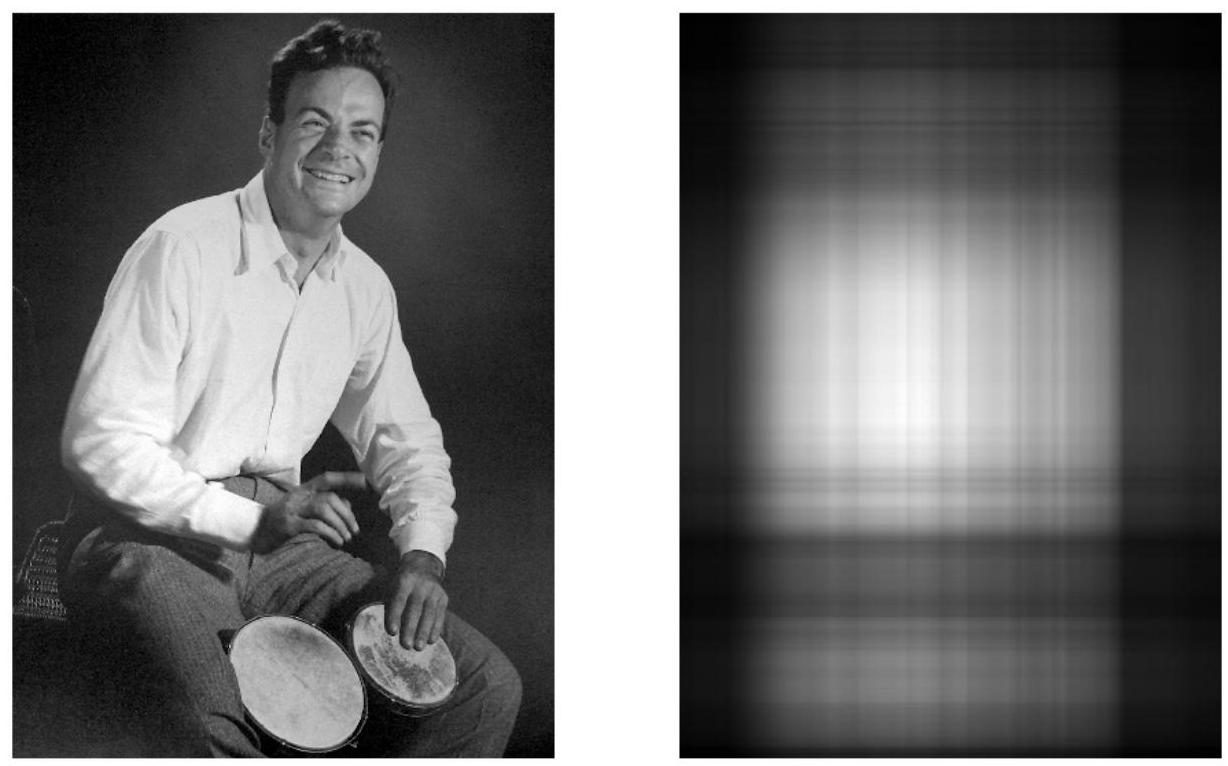
\includegraphics[max width=\textwidth, center]{2024_04_17_aea350b0a5e2209a42f2g-03}

Figure 1: Feynman playing the bongos, and his rank-1 approximation. The approximate Feynman is clearly the product of one profile $\boldsymbol{u}_{1}$ in the vertical direction, and one, $\boldsymbol{v}_{1}^{\top}$, in the horizontal. The Frobenius error of the approximation is only $36.5 \%$.

\section*{3 Bipartite entanglement}
\subsection*{3.1 Schmidt decomposition}
The SVD has a direct implication that is crucial to our efforts to efficiently study quantum wavefunctions. Consider a state $|\psi\rangle$ of a system with open boundary conditions which can be partitioned into a subsystem $\mathcal{A}$ and its complement $\mathcal{A}^{c}$, with Hilbert space $\mathcal{H}=\mathcal{H}_{\mathcal{A}} \otimes \mathcal{H}_{\mathcal{A}^{c}}$. Let $\mathcal{H}_{\mathcal{A}}$ be spanned by $\left|a_{i}\right\rangle, i=1, \ldots, \operatorname{dim}\left(\mathcal{H}_{\mathcal{A}}\right)$, and $\mathcal{H}_{\mathcal{A}^{c}}$ by $\left|b_{j}\right\rangle, j=1, \ldots, \operatorname{dim}\left(\mathcal{H}_{\mathcal{A}^{c}}\right)$. Naively, one would expect that\\
the simplest general way to write the wavefunction is


\begin{equation*}
|\psi\rangle=\sum_{i, j} c_{i j}\left|a_{i}\right\rangle \otimes\left|b_{j}\right\rangle \tag{4}
\end{equation*}


Written in this way, $|\psi\rangle$ can be associated with a bilinear operator through a formal procedure of matricization $\mathfrak{M}$ that simply amounts to $\left|b_{j}\right\rangle \rightarrow\left\langle b_{j}\right|$, which is evidently a bijection:


\begin{equation*}
|\psi\rangle=\sum_{i, j} c_{i j}\left|a_{i}\right\rangle\left|b_{j}\right\rangle \quad \xrightarrow{\mathfrak{M}} \quad M_{|\psi\rangle}=\sum_{i, j} c_{i j}\left|a_{i}\right\rangle\left\langle b_{j}\right| \tag{5}
\end{equation*}


`   `Now we have $M_{|\psi\rangle}, \operatorname{adim}\left(\mathcal{H}_{\mathcal{A}}\right) \times \operatorname{dim}\left(\mathcal{H}_{\mathcal{A}^{c}}\right)$ matrix, and the SVD obtains a basis $\left|u_{\alpha}\right\rangle, \alpha=1, \ldots, r$, for $\mathcal{H}_{\mathcal{A}}$ and corresponding basis $\left|v_{\alpha}\right\rangle$ for $\mathcal{H}_{\mathcal{A}^{c}}$, where $r=\min \left(\operatorname{dim}\left(\mathcal{H}_{\mathcal{A}}\right), \operatorname{dim}\left(\mathcal{H}_{\mathcal{A}^{c}}\right)\right)$, permitting


\begin{equation*}
M_{|\psi\rangle}=\sum_{\alpha=1}^{r} \lambda_{\alpha}\left|u_{\alpha}\right\rangle\left\langle v_{\alpha}\left|\xrightarrow{\mathfrak{M}^{-1}}\right| \psi\right\rangle=\sum_{\alpha=1}^{r} \lambda_{\alpha}\left|u_{\alpha}\right\rangle \otimes\left|v_{\alpha}\right\rangle \tag{6}
\end{equation*}


The singular values $\lambda_{\alpha}$ of $M_{|\psi\rangle}$ are called the Schmidt values of the state $|\psi\rangle$, and the orthonormal basis states are left or right $S$ chmidt vectors.

We can approximate the state $|\psi\rangle$ by reducing the Schmidt rank to $k$ across the cut, throwing away the smallest $r-k$ Schmidt vectors. However, as this is a quantum wavefunction, we must be careful to maintain normalization. Initially, $\langle\psi \mid \psi\rangle=\sum_{\alpha, \alpha^{\prime}} \lambda_{\alpha} \lambda_{\alpha^{\prime}}\left\langle u_{\alpha^{\prime}} \mid u_{\alpha}\right\rangle\left\langle v_{\alpha^{\prime}} \mid v_{\alpha}\right\rangle=\sum_{\alpha} \lambda_{\alpha}^{2}=1$, and as the norm of the approximate state is


\begin{equation*}
\sqrt{\langle\tilde{\psi} \mid \tilde{\psi}\rangle}=\sqrt{\sum_{\alpha=1}^{k} \lambda_{\alpha}^{2}}=\sqrt{1-\sum_{\alpha=k+1}^{r} \lambda_{\alpha}^{2}} \tag{7}
\end{equation*}


the state is normalized by rescaling all remaining Schmidt values by this amount.

\subsection*{3.2 Entanglement entropy}
The general form (6) of a bipartite wavefunction reveals a great deal of information about the relationship between the two subsystems. If and only if $r=1$ (that is, the only nonzero Schmidt value is $\lambda_{1}=1$ ), then $|\psi\rangle$ is a product state between $\mathcal{A}$ and $\mathcal{A}^{c}$, and is unentangled across the boundary. If $r>1$ there is some degree of entanglement, which we can quantify in a natural way. Consider the following Schmidt decomposition parameterizing a manifold of states with $r=2$ : $|\psi(t)\rangle=\sqrt{1-t}\left|u_{1}\right\rangle\left|v_{1}\right\rangle+\sqrt{t}\left|u_{2}\right\rangle\left|v_{2}\right\rangle$, with $t \in[0,1 / 2]$. If $t=\epsilon \ll 1$, the subsystems are nearly uncorrelated, and an observable of the following form almost factorizes:


\begin{equation*}
\left\langle\psi(\epsilon)\left|O_{\mathcal{A}} \otimes O_{\mathcal{A}^{c}}\right| \psi(\epsilon)\right\rangle=\left\langle u_{1}\left|O_{\mathcal{A}}\right| u_{1}\right\rangle\left\langle v_{1}\left|O_{\mathcal{A}^{c}}\right| v_{1}\right\rangle+\mathcal{O}(\epsilon) . \tag{8}
\end{equation*}


This can be understood visually by referencing Fig. 1, in which the approximate image clearly factorizes into the vertical and horizontal directions. A small perturbation would cause only a small change. On the other hand, for $t=1 / 2$ the state is an equally weighted superposition of terms, and is as far from factorizable as is possible since one cannot designate either term as dominant. Accordingly, the state is said to be maximally entangled for $t=1 / 2$.

We can make the preceding discussion more precise using an idea from information theory.

Specifically, recalling that $\sum_{\alpha} \lambda_{\alpha}^{2}=1$, we can regard $p(\alpha)=\lambda_{\alpha}^{2}$ as a discrete probability distribution. Then the notion described above corresponds to the Shannon entropy of the distribution:


\begin{equation*}
H[p]=-\sum_{\alpha} p(\alpha) \log p(\alpha) \Longrightarrow S=-\sum_{\alpha} \lambda_{\alpha}^{2} \log \lambda_{\alpha}^{2} \tag{9}
\end{equation*}


The quantity $S$ is called entanglement entropy, and is well-defined for a state $|\psi\rangle$ and specified bipartition, because the Schmidt spectrum is unique.

In the example above, $S(|\psi(0)\rangle)=0$ indicates a product state and $S(|\psi(1 / 2)\rangle)=\log 2$ a maximally entangled state (under the constraint $r=2$ ). These results generalize naturally. Remember that for a given bipartition $\left(\mathcal{A}, \mathcal{A}^{c}\right)$ of a system, the $\operatorname{Schmidt}$ rank is $r=\min \left(\operatorname{dim}\left(\mathcal{H}_{\mathcal{A}}\right), \operatorname{dim}\left(\mathcal{H}_{\mathcal{A}^{c}}\right)\right)$; then product states have $S=0$, and for maximally entangled states $S=\log r$. These values bound the entanglement entropy of all possible quantum states under this bipartition.

\subsection*{3.3 Scaling of entanglement entropy}
So far the discussion of entanglement entropy has been a bit abstract, but this quantity is in fact closely related to the physics of a many-body quantum system. To make this connection, we consider $S(\ell)$, where $\ell=|\mathcal{A}| \leq\left|\mathcal{A}^{c}\right|$ (without loss of generality; $S$ is invariant under $\mathcal{A} \leftrightarrow \mathcal{A}^{c}$ ), and $\mathcal{A}$ is contiguous. The scaling of $S(\ell)$ with $\ell$ in ground states depends strongly on the nature of the Hamiltonian, and in fact reveals some of its fundamental properties. The proofs of these results - those that are known - are difficult, and we will argue from simpler physical grounds.

The naive bound on entanglement entropy depends on the dimension of $\mathcal{H}_{\mathcal{A}}$. From the previous section, a maximally entangled state has


\begin{equation*}
S(\ell)=\log r=\log \operatorname{dim}\left(\mathcal{H}_{\mathcal{A}}\right)=\log \operatorname{dim}\left(\left(\mathbb{C}^{d}\right)^{\otimes \ell}\right)=\ell \log d \tag{10}
\end{equation*}


That is, $S \sim \ell$. This is referred to as volume law entanglement scaling, which is saturated by typical states in the many-body Hilbert space. This includes highly-excited eigenstates away from the band edges of local Hamiltonians, as these generically do not avoid typicality.

However, sub-volume law entanglement scaling applies to ground states of local Hamiltonians with a finite excitation gap $\Delta$ in the thermodynamic limit. This is a consequence of a finite correlation length $\xi \sim 1 / \Delta$ which controls the exponential decay of correlations between spatially separated observables. Because only degrees of freedom in $\mathcal{A}$ that are close (relative to $\xi$ ) to the boundary $\partial \mathcal{A}$ can be correlated with the complement, those degrees of freedom sufficiently far away contribute no entanglement under this bipartition. Therefore we expect the entanglement entropy to scale not as $\ell=|\mathcal{A}|$ but instead with the size of the boundary, $|\partial \mathcal{A}|$. In one dimension, $\partial \mathcal{A}$ is simply the endpoints of $\mathcal{A}$; thus $S(\ell) \sim \kappa(\xi)$, independent of $\ell$ for large $\ell>\xi$. This result is known as the area law of entanglement, and was proved by Matt Hastings in 2007. It formalizes the notion that ground states occupy a specialized and extremely small region of Hilbert space.

More exotic entanglement scaling is exhibited by ground states of Hamiltonians tuned to critical points. Here there is no energy gap, and accordingly the correlation length diverges. There is no length scale above which the system can be considered trivial, and at long distances the system displays scale invariance. A scale-invariant theory in one dimension is also conformally invariant, and is described by the technology of conformal field theory (CFT), in which correlation functions decay according to power laws and distant lattice sites do indeed contribute to entanglement. The scaling of entanglement entropy in a CFT was calculated by Calabrese and Cardy in 2004, who found a relatively mild logarithmic violation of the area law, given in the thermodynamic limit by $S(\ell) \sim \frac{c}{3} \log \ell$ to leading order. In the finite periodic case the logarithmic violation remains but is corrected to use the chord length: $S(\ell) \sim \frac{c}{3} \log \left(\frac{L}{\pi} \sin \frac{\pi \ell}{L}\right)$, demonstrating the entanglement entropy's long-range knowledge of the system.

In contrast to the gapped case where $\kappa$ depends on $\xi$, the coefficient for critical entanglement scaling is universal: $c$ is the "central charge," an important characterization of the CFT describing

the critical point. Central charges are known for many CFTs; in particular, $c=1 / 2$ for free fermions and $c=1$ for free bosons. Note that these emergent descriptions do not necessarily\\
mirror the lattice theory: for example, the Heisenberg model of spins-which maps to microscopic fermions - is described at low energies by a free boson CFT.

As a final remark, one might question the statement of a necessarily finite correlation length in gapped systems, based on the asymptotically finite value of $\left\langle\sigma_{1}^{z} \sigma_{1+r}^{z}\right\rangle$ in the ordered phase of the quantum Ising model. Previously it was claimed that the true ground state is $\sim|\uparrow \uparrow \cdots \uparrow\rangle+|\downarrow \downarrow \cdots \downarrow\rangle$, which respects the Ising symmetry. But this state, which has Schmidt rank $r=2$ across all cuts, is clearly long-range entangled and in the thermodynamic limit is a macroscopic superposition state, which is not observed in nature. What happens is that as $L \rightarrow \infty$, fluctuations spontaneously choose one of the degenerate symmetry-breaking product states and the connected correlation function $C_{\text {conn }}^{z z}(r)=\left\langle\sigma_{1}^{z} \sigma_{1+r}^{z}\right\rangle-\left\langle\sigma_{1}^{z}\right\rangle\left\langle\sigma_{1+r}^{z}\right\rangle$ which detects quantum correlations indeed decays exponentially. However, there is a signature of the twofold ground state degeneracy in the entanglement entropy, in the form of a subleading term: a constant $\log 2$ in the ferromagnet phase.

\section*{4 Matrix product states}
\subsection*{4.1 Compressing an ED wavefunction into an MPS}
We will utilize the SVD and the physical principles of entanglement scaling to write quantum states in an extremely compact form known as a matrix product state (MPS). This will eventually allow us to extend our simulations to much larger system sizes. The MPS is an ansatz suitable for wavefunctions in one dimension which follow an area law; although this is true for vanishingly few states, it does apply to the ground states (and low-energy eigenstates) of local Hamiltonians.

Following Sec. 3.2, we may consider one-dimensional systems with open boundary conditions to be bipartite, with a boundary consisting of a single bond between two neighboring lattice sites. Performing the Schmidt decomposition exposes the entanglement across this bond, and according to the area law the Schmidt rank $r$ is much less than its theoretical maximum and is in fact bounded by some constant $\chi$. An MPS is obtained by repeating the bipartition between every pair of neighboring sites, relying each time on the strong bound on the number of Schmidt values. Initially the wavefunction can be written


\begin{equation*}
|\psi\rangle=\sum_{\sigma_{1}, \ldots, \sigma_{L}} C_{\sigma_{1}, \ldots, \sigma_{L}}\left|\sigma_{1}, \ldots, \sigma_{L}\right\rangle \tag{11}
\end{equation*}


where the tensor of coefficients $C$ has $L$ indices for the spin degrees of freedom $\sigma_{i}, i=1, \ldots, L$. We partition the system into regions $\mathcal{A}=\left\{\sigma_{1}\right\}$ and $\mathcal{A}^{c}=\left\{\sigma_{2}, \ldots, \sigma_{L}\right\}$, and apply the matricization of Sec. 3.1 to $|\psi\rangle$, using parentheses to indicate grouping of the indices of $C$. Performing an SVD,


\begin{equation*}
C_{\sigma_{1},\left(\sigma_{2}, \ldots, \sigma_{L}\right)}=\sum_{\alpha} U_{\sigma_{1}, \alpha} S_{\alpha, \alpha}\left(V^{\dagger}\right)_{\alpha,\left(\sigma_{2}, \ldots, \sigma_{L}\right)} \tag{12}
\end{equation*}


where $\operatorname{dim}(\alpha) \leq \chi$. We rename $U_{\sigma_{1}, \alpha}=\left(A^{1}\right)_{\alpha}^{\sigma_{1}}$ and multiply the diagonal matrix into $V^{\dagger}$ to obtain $W_{\alpha,\left(\sigma_{2}, \ldots, \sigma_{L}\right)} \equiv S_{\alpha, \alpha}\left(V^{\dagger}\right)_{\alpha,\left(\sigma_{2}, \ldots, \sigma_{L}\right)}$. Applying inverse matricization, the state is rewritten


\begin{align*}
M_{|\psi\rangle} & =\sum_{\sigma_{1}, \ldots, \sigma_{L}} \sum_{\alpha}\left(A^{1}\right)_{\alpha}^{\sigma_{1}} W_{\alpha,\left(\sigma_{2}, \ldots, \sigma_{L}\right)}\left|\sigma_{1}\right\rangle\left\langle\sigma_{2}, \ldots, \sigma_{L}\right|  \tag{13}\\
& \xrightarrow{\mathfrak{M}^{-1}}|\psi\rangle=\sum_{\sigma_{1}, \ldots, \sigma_{L}} \sum_{\alpha}\left(A^{1}\right)_{\alpha}^{\sigma_{1}} W_{\alpha, \sigma_{2}, \ldots, \sigma_{L}}\left|\sigma_{1}, \ldots, \sigma_{L}\right\rangle \tag{14}
\end{align*}


Now simply iterate the process, regrouping the spin indices on $W$ to expose $\sigma_{2}$, which is grouped with the Schmidt index from the previous cut, applying $\mathfrak{M}$, and performing another SVD:


\begin{equation*}
W_{\alpha, \sigma_{2}, \ldots, \sigma_{L}} \xrightarrow{\mathfrak{M}} W_{\left(\alpha, \sigma_{2}\right),\left(\sigma_{3}, \ldots, \sigma_{L}\right)}=\sum_{\beta} U_{\left(\alpha, \sigma_{2}\right), \beta} S_{\beta, \beta}\left(V^{\dagger}\right)_{\beta,\left(\sigma_{3}, \ldots, \sigma_{L}\right)} \tag{15}
\end{equation*}


Again relabel $U_{\left(\alpha, \sigma_{2}\right), \beta}=\left(A^{2}\right)_{\alpha, \beta}^{\sigma_{2}}$ and $W_{\beta,\left(\sigma_{3}, \ldots, \sigma_{L}\right)} \equiv S_{\beta, \beta}\left(V^{\dagger}\right)_{\beta,\left(\sigma_{3}, \ldots, \sigma_{L}\right)}$ and apply $\mathfrak{M}^{-1}$. At the next step, you will reshape (matricize) this new $W: W_{\beta,\left(\sigma_{3}, \sigma_{4}, \ldots, \sigma_{L}\right)} \rightarrow W_{\left(\beta, \sigma_{3}\right),\left(\sigma_{4}, \ldots, \sigma_{L}\right)}$ and SVD this, and so on. At each step, we can use the singular values to truncate the bond dimension by keeping only $\chi$ leading singular values. After $L-1$ steps we eventually obtain the following form of the state:


\begin{equation*}
|\psi\rangle=\sum_{\sigma_{1}, \ldots, \sigma_{L}} \sum_{\alpha, \beta, \ldots, \omega}\left(A^{1}\right)_{\alpha}^{\sigma_{1}}\left(A^{2}\right)_{\alpha, \beta}^{\sigma_{2}} \cdots\left(A^{L}\right)_{\omega}^{\sigma_{L}}\left|\sigma_{1}, \ldots, \sigma_{L}\right\rangle \tag{16}
\end{equation*}


This is the MPS representation of $|\psi\rangle$. At the last step $\left(A^{L}\right)_{\omega}^{\sigma_{L}} \equiv S_{\omega, \omega}\left(V^{\dagger}\right)_{\omega, \sigma_{L}}$. Counting the dimension of each index shows that the MPS form of $|\psi\rangle$ uses at most $2 \chi^{2}(L-2)+4 \chi$ coefficients to represent the state exactly, an exponential reduction compared to (11).

\subsection*{4.2 Performing calculations with MPS}
In this section we draw heavily from Ch. 4 of [1. The benefit of MPS is not only its concise description of certain quantum states; it also turns out to be a useful platform for many interesting physical calculations like overlaps, matrix elements, and correlations. These operations are conveniently described by the graphical calculus of tensor networks, a formalism for performing summations over many indices, as in (16). For example, computing the overlap between states $\langle\phi \mid \psi\rangle$, where $|\phi\rangle$ has $B$-tensors, one finds


\begin{equation*}
\langle\phi \mid \psi\rangle=\sum_{\sigma_{1}, \ldots, \sigma_{L}} \sum_{\alpha, \beta, \ldots, \omega} \sum_{\alpha^{\prime}, \beta^{\prime}, \ldots, \omega^{\prime}}\left(B^{L \dagger}\right)_{\omega^{\prime}}^{\sigma_{L}} \cdots\left(B^{2 \dagger}\right)_{\beta^{\prime}, \alpha^{\prime}}^{\sigma_{2}}\left(B^{1 \dagger}\right)_{\alpha^{\prime}}^{\sigma_{1}}\left(A^{1}\right)_{\alpha}^{\sigma_{1}}\left(A^{2}\right)_{\alpha, \beta}^{\sigma_{2}} \cdots\left(A^{L}\right)_{\omega}^{\sigma_{L}} \tag{17}
\end{equation*}


Instead of continuing in this way, we draw diagrams with each tensor represented by a filled shape and attached legs corresponding to each tensor index. A scalar has no legs, a vector one leg, a matrix two legs, and so on. Summation is indicated between two tensors by connecting the legs representing the index to be summed over. The process of performing sums over indices in a tensor network diagram is called contraction. Thus, Fig. 2 reproduces (16): summation over virtual indices arising from the SVD by contracting the appropriate legs on adjacent tensors. The imposition of physical spin configurations is implicitly understood from the uncontracted physical legs.\\
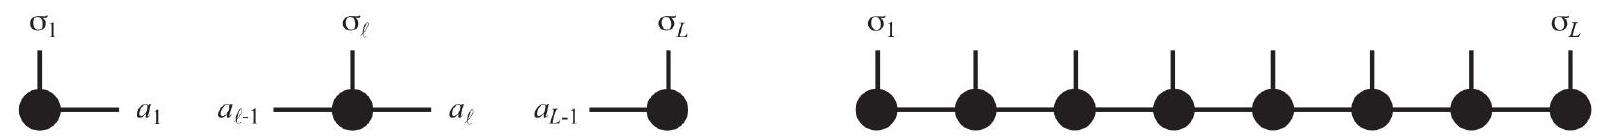
\includegraphics[max width=\textwidth, center]{2024_04_17_aea350b0a5e2209a42f2g-07}

Figure 2: Figures taken from [1]. By convention when writing MPS, physical indices $\sigma_{i}$ point vertically and virtual indices (here, $a_{1}, a_{2}, \ldots$ ) connect horizontally. The lefthand diagram shows the tensors $A^{1}, A^{\ell}, A^{L}$, with no operation performed, and the righthand diagram replicates (16).

Now we return to the problem of the overlap (17). Because $\langle\phi \mid \psi\rangle$ is a scalar quantity the diagram we draw can have no uncontracted indices, including physical legs. In order to indicate Hermitian conjugation we flip the tensors vertically, so the physical indices of $\langle\phi|$ point downward. Now the form in Fig. 3 should suggest itself; the contracted vertical legs are the spin indices $\sigma_{i}$, and\\
the contracted top and bottom horizontal legs are the virtual indices $\alpha^{\prime}, \beta^{\prime}, \ldots, \omega^{\prime}$ on $B^{\dagger}$-tensors and $\alpha, \beta, \ldots, \omega$ on $A$-tensors. In the case that $\langle\phi|=\langle\psi|$, the tensor network in Fig. 3 computes the squared norm $\langle\psi \mid \psi\rangle$, which can be used for normalization in other computations.

\begin{center}
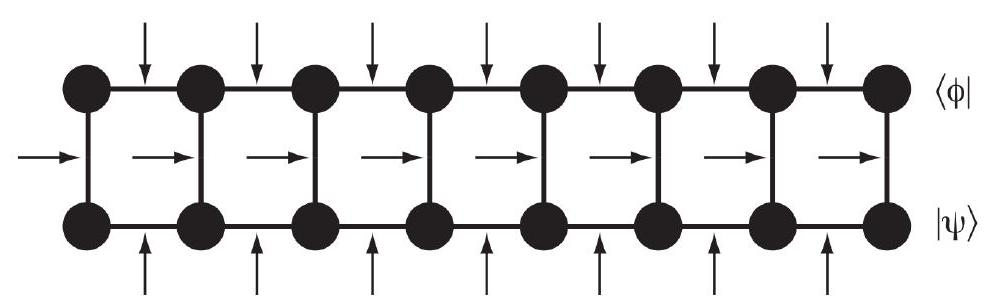
\includegraphics[max width=\textwidth]{2024_04_17_aea350b0a5e2209a42f2g-08(1)}
\end{center}

Figure 3: Figure taken from [1]. This is the tensor network for the overlap (17), with arrows pointing to all of the indices $\left\{\sigma_{1}, \ldots, \sigma_{L}\right\},\{\alpha, \beta, \ldots, \omega\},\left\{\alpha^{\prime}, \beta^{\prime}, \ldots, \omega^{\prime}\right\}$ which are summed over in the contraction. The top row of tensors are the $\left(B^{j}\right)^{\dagger}$ in (17), and the bottom the $A^{j}$.

A generalization of the tensor network for overlaps allows us to easily compute matrix elements of local observables. Recall that some local observable $O(j)$ acting on site $j$ may be written $O_{j}=\sum_{\sigma_{j}, \sigma_{j}^{\prime}} O^{\sigma_{j}^{\prime}, \sigma_{j}}\left|\sigma_{j}^{\prime}\right\rangle\left\langle\sigma_{j}\right|$, where $\sigma_{j}^{\prime}$ is the same degree of freedom as $\sigma_{j}$ but distinguished by belonging to the adjoint state. In the tensor network, we need only insert the matrix for $O_{j}$ into the contraction at the appropriate location, now performing a double sum over $\sigma_{j}$ and $\sigma_{j}^{\prime}$ since we do not find the factor $\delta_{\sigma_{j}^{\prime}}^{\sigma_{j}}$ that was used to obtain (17). This generalizes to products of local observables, as shown in Fig. 4 which computes the matrix element $\left\langle\phi\left|O_{j} O_{k}\right| \psi\right\rangle$. Because the Hamiltonian is a sum of local terms, by adding the results of multiple contracted tensor networks we can compute the matrix element $\langle\phi|H| \psi\rangle$.

\begin{center}
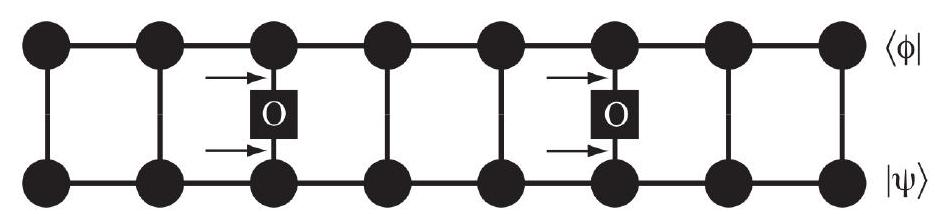
\includegraphics[max width=\textwidth]{2024_04_17_aea350b0a5e2209a42f2g-08}
\end{center}

Figure 4: Figure taken from [1. Each of the lines connecting the spin indices $\sigma_{j}$ can be thought of as a delta function $\delta_{\sigma_{j}^{\prime}}^{\sigma_{j}}$; in this sense, the network in Fig. 3 computes the matrix element of the identity $\mathbb{I}=\mathbb{I}_{1} \otimes \cdots \otimes \mathbb{I}_{L}$. In this diagram we compute a matrix element of the more general observable $O_{j} O_{k}$.

\subsection*{4.3 Practical considerations in tensor network contraction}
The outcome of a contraction is independent of the order in which the sums are performed, but for practical reasons some patterns are clearly preferred. For example, by contracting virtual indices first we again obtain tensors with $2^{L}$ coefficients, which eliminates the benefits of using MPS. In general, optimal contraction of tensor networks is known to be an NP-complete problem. However for MPS the task is simpler, and we can define a general procedure that is nearly optimal. By

contracting the tensors vertically at a site $j$-that is, $\left(A^{j}\right)^{\sigma_{j}},\left(B^{j}\right)^{\sigma_{j}^{\prime}}$, and $O_{j}$ if applicable - we obtain a 4-tensor of dimension $\chi^{4}$. This is not too large, so we can do so at each site, then starting from the left contract the virtual indices $\left(\alpha, \alpha^{\prime}\right)$, then $\left(\beta, \beta^{\prime}\right)$, and so on. Because the cost of each vertical contraction does not depend on the system size and the number of horizontal contractions\\
scales as $L$, this "vertical-first" pattern scales linearly with system size. This is an efficient enough strategy to use on computers, and is clearly far superior to the exponential scaling of ED operations.

\subsection*{4.4 Canonical form for MPS}
This is a more technical material to make some preparations for the most challenging Assignment 4 (the text and this part of the assignment is not polished - added this year to make the Assignment 4 easier later - suggestions for improvements are welcome!). Consider a chain of length $L$ with open boundary conditions and a quantum state in the MPS form,


\begin{align*}
& |\psi\rangle=\sum_{\sigma_{1}, \sigma_{2}, \ldots, \sigma_{L}} c_{\sigma_{1}, \sigma_{2}, \ldots, \sigma_{L}}\left|\sigma_{1}, \sigma_{2}, \ldots, \sigma_{L}\right\rangle  \tag{18}\\
& c_{\sigma_{1}, \sigma_{2}, \ldots, \sigma_{L}}=\sum_{a_{1}, a_{2}, \ldots, a_{L-1}} A_{a_{1}}^{(1) \sigma_{1}} A_{a_{1}, a_{2}}^{(2) \sigma_{2}} \ldots A_{a_{\ell-1}, a_{\ell}}^{(\ell) \sigma_{\ell}} \ldots A_{a_{L-2}, a_{L-1}}^{(L-1) \sigma_{L-1}} A_{a_{L-1}}^{(L) \sigma_{L}} . \tag{19}
\end{align*}


(For some later formulas to make the left end look similar to "bulk", it is convenient to introduce $a_{0}$ taking only a single value $a_{0}=1$ and write the first factor as $A_{a_{1}}^{(1) \sigma_{1}} \equiv A_{a_{0}=1, a_{1}}^{(1) \sigma_{1}}$; and similarly for the right end.) As sketched in previous subsections and detailed in the notes, efficient calculations with MPS can be formulated using so-called "transfer matrices" (a.k.a., "double-tensor")


\begin{equation*}
E_{\left(a_{\ell-1}^{\prime}, a_{\ell-1}\right),\left(a_{\ell}^{\prime}, a_{\ell}\right)}^{(\ell)} \equiv \sum_{\sigma_{\ell}}\left(A_{a_{\ell-1}^{\prime}, a_{\ell}^{\prime}}^{(\ell) \sigma_{\ell}}\right)^{*} A_{a_{\ell-1}, a_{\ell}}^{(\ell) \sigma_{\ell}} \tag{20}
\end{equation*}


Using transfer matrices already reduces the computational costs with $|\psi\rangle$ from exponential in $L$ to $\sim L \chi^{2}$ (where $\chi$ is the bond dimension), but this can be even further reduced using so-called "canonical forms" for the MPS that make the transfer matrices particularly simple to use and are also important for other purposes. The most useful canonical form is so-called "canonical form with an orthogonality center", say, located between sites $j$ and $j+1$, and stated as follows:


\begin{equation*}
c_{\sigma_{1}, \sigma_{2}, \ldots, \sigma_{L}}=\sum_{a_{1}, a_{2}, \ldots, a_{L-1}} A_{a_{1}}^{(1) \sigma_{1}} A_{a_{1}, a_{2}}^{(2) \sigma_{2}} \ldots A_{a_{j-1}, a_{j}}^{(j) \sigma_{j}} S_{a_{j}, a_{j}} A_{a_{j}, a_{j+1}}^{(j+1) \sigma_{j+1}} \ldots A_{a_{L-2}, a_{L-1}}^{(L-1) \sigma_{L-1}} A_{a_{L-1}}^{(L) \sigma_{L}} \tag{21}
\end{equation*}


with $A^{(\ell) \sigma_{\ell}}$ matrices satisfying


\begin{align*}
& \text { left-canonical condition for } \ell \leq j: \quad \sum_{\sigma_{\ell}}\left(A^{(\ell) \sigma_{\ell}}\right)^{\dagger} A^{(\ell) \sigma_{\ell}}=1,  \tag{22}\\
& \text { right-canonical condition for } \ell \geq j+1: \quad \sum_{\sigma_{\ell}} A^{(\ell) \sigma_{\ell}}\left(A^{(\ell) \sigma_{\ell}}\right)^{\dagger}=1,  \tag{23}\\
& \text { non-negative diagonal matrix : } \quad S_{a_{j}, a_{j}} \geq 0 \text { (Schmidt values). } \tag{24}
\end{align*}


The above form is slightly different from the standard MPS form because of the extra diagonal matrix $S$, but this can be recast into the standard form by redefining either $A^{(j)}$ or $A^{(j+1)}$ matrices "multiplying" $S$ into them. See the notes for the left- and right-canonicity conditions written out with all indices spelled out, and also for the simplifications in calculations of the wavefunction normalization and expectation values of observables at $j$. What is most important for us is that this canonical form immediately gives Schmidt values for the Schmidt decomposition across the cut between $j$ and $j+1$ as $S_{a_{j}, a_{j}}$, see the notes for details.

For any state, we can calculate the Schmidt values across any cut by expanding the state in the full computational basis $\left|\sigma_{1}, \sigma_{2}, \ldots, \sigma_{L}\right\rangle$ and performing SVD as described earlier. However,\\
if we have a state in an MPS form, we can achieve the calculation of the Schmidt values without ever expanding in the full computational basis by using a procedure that brings the MPS into the canonical form as follows. (Note that the original MPS need not be in the canonical form; e.g., when we act on a trial MPS with a Hamiltonian as we will do in Assignment 4, the result can be written as an MPS, but any canonical form is usually lost and needs to be restored for consistent truncations guided by the true Schmidt values of the wavefunction.) We first sweep from the left end to the right. Suppose matrices $A^{(1)}, \ldots, A^{(\ell-1)}$ are already left-canonical. Next we turn $A^{(\ell)}$ left-canonical by doing SVD of the following matrix:


\begin{equation*}
W_{\left(a_{\ell-1}, \sigma_{\ell}\right),\left(\sigma_{\ell+1}, a_{\ell+1}\right)} \equiv \sum_{a_{\ell}} A_{a_{\ell-1}, a_{\ell}}^{(\ell) \sigma_{\ell}} A_{a_{\ell}, a_{\ell+1}}^{(\ell+1) \sigma_{\ell+1}}=\sum_{k} U_{\left(a_{\ell-1}, \sigma_{\ell}\right), k} S_{k k}\left(V^{\dagger}\right)_{k,\left(\sigma_{\ell+1}, a_{\ell+1}\right)} \tag{25}
\end{equation*}


where the last equation is the result of the SVD. A reshaped $U$ becomes the new $\tilde{A}^{(\ell)}$ [specifically, $\left.\tilde{A}_{a_{\ell-1}, k}^{(\ell), \sigma_{\ell}} \equiv U_{\left(a_{\ell-1}, \sigma_{\ell}\right), k}\right]$ satisfying the left canonicity condition, while a reshaped $V$ with $S_{k k}$ 's absorbed into it become the new $\tilde{A}^{(\ell+1)}$ [specifically, $\tilde{A}_{k, a_{\ell+1}}^{(\ell+1) \sigma_{\ell+1}} \equiv S_{k k} V_{\left(\sigma_{\ell+1}, a_{\ell+1}\right), k}^{*}$ ]. Dropping tildes on $\tilde{A}^{(\ell)}, \tilde{A}^{(\ell+1)}$, we now have matrices $A^{(1)}, \ldots A^{(\ell-1)}, A^{(\ell)}$ as left-canonical, and we then move to the next site $\ell+1$. Note that the $S_{k k}$ 's we find at each step are NOT Schmidt values for the wavefunction, since we really are not using information about the wavefunction outside the treated two-site blocks, and the rest of the matrices to the right are not right-canonical. Only at the very last step of the sweep when we are treating the block $(\ell, \ell+1)=(L-1, L)$ the resulting $\tilde{A}^{(\ell+1)}$ is the only matrix to the right and is right-canonical (if we are keeping $S_{k k}$ 's separate at this step); hence only at this point during the sweep the $S_{k k}$ 's are Schmidt values for the cut between $L-1$ and $L$, and we have succeeded to obtain the canonical form with the orthogonality center between $L-1$ and $L$. Now we can actually move the orthogonality center to any position (between $j$ and $j+1$ on the chain) by sweeping from the right end to the left making the matrices $A^{(L)}, A^{(L-1)}, \ldots, A^{(j+1)}$ as right-canonical. In this sweep, at each step the generated $S_{k k}$ 's are the true Schmidt values for the whole wavefunction; when we perform the sweep since we are moving to the left keeping the right matrices right-canonical, we absorb these $S_{k k}$ 's by multiplying them into the left matrices of the SVD at each step. The procedure involves a lot of re-shaping ("matricizing") of tensors and book-keeping, and we will practice it on a simple example in this Assignment.

\section*{5 Assignment: entanglement entropy and state compression}
\subsection*{5.1 Image compression}
Select a few grayscale images and treat each as a real-valued matrix, compressing using the SVD. For each image, use approximations of various rank, e.g., $k=\{n / 4, n / 8, n / 16, n / 32, \ldots\}$, where $n$ is the smaller image dimension. Show some examples of images that compress well, and poorly, and compute the Frobenius distance (or "discarded norm") between the compressed images and the originals: $d(k)=\|\tilde{A}(k)-A\|_{F}$, where $\tilde{A}(k)$ is the rank- $k$ approximation to image $A$. You may also use the singular value spectrum as a guide to truncation if there are evident features. What reduction in storage space are you able to achieve without too badly degrading the image?
\newpage
% Inline Python code in the document
\begin{lstlisting}[language=Python]
import numpy as np
import matplotlib.pyplot as plt
from skimage import img_as_float
import os

print(os.getcwd())

def load_and_convert_image(image_path):
    image = plt.imread(image_path)
    return img_as_float(image)

# define the image paths
image_path = 'hw2/src/parrot.png'

# load and convert the image
image = load_and_convert_image(image_path)
print(image.shape)
# perform the svd on the image


def reconstruct_image(U, s, Vt, k):
    S_k = np.diag(s[:k])
    U_k = U[:, :k]
    Vt_k = Vt[:k, :]
    return np.dot(U_k, np.dot(S_k, Vt_k))

def calculate_frobenius_norms(image_path, ranks):
    image = load_and_convert_image(image_path)
    U, s, Vt = np.linalg.svd(image, full_matrices=False)
    originals = [reconstruct_image(U, s, Vt, k) for k in ranks]
    frobenius_norms = [np.linalg.norm(original - image, 'fro') for original in originals]
    return originals, frobenius_norms

smaller_dim = min(image.shape)
# the ranks go like smaller_dim/(2^i) for i in range(0, 8)
ranks = [smaller_dim // (2**i) for i in range(8)]
reconstructions, frobenius_norms = calculate_frobenius_norms(image_path, ranks)
# show the images corresponding to the reconstructions
fig, axes = plt.subplots(2, 4, figsize=(20, 10))
for i, ax in enumerate(axes.flatten()):
    ax.imshow(reconstructions[i])
    ax.set_title(f'k = {ranks[i]}')
    ax.axis('off')
plt.savefig('reconstructions.png')

\end{lstlisting}
\begin{figure}
\centering
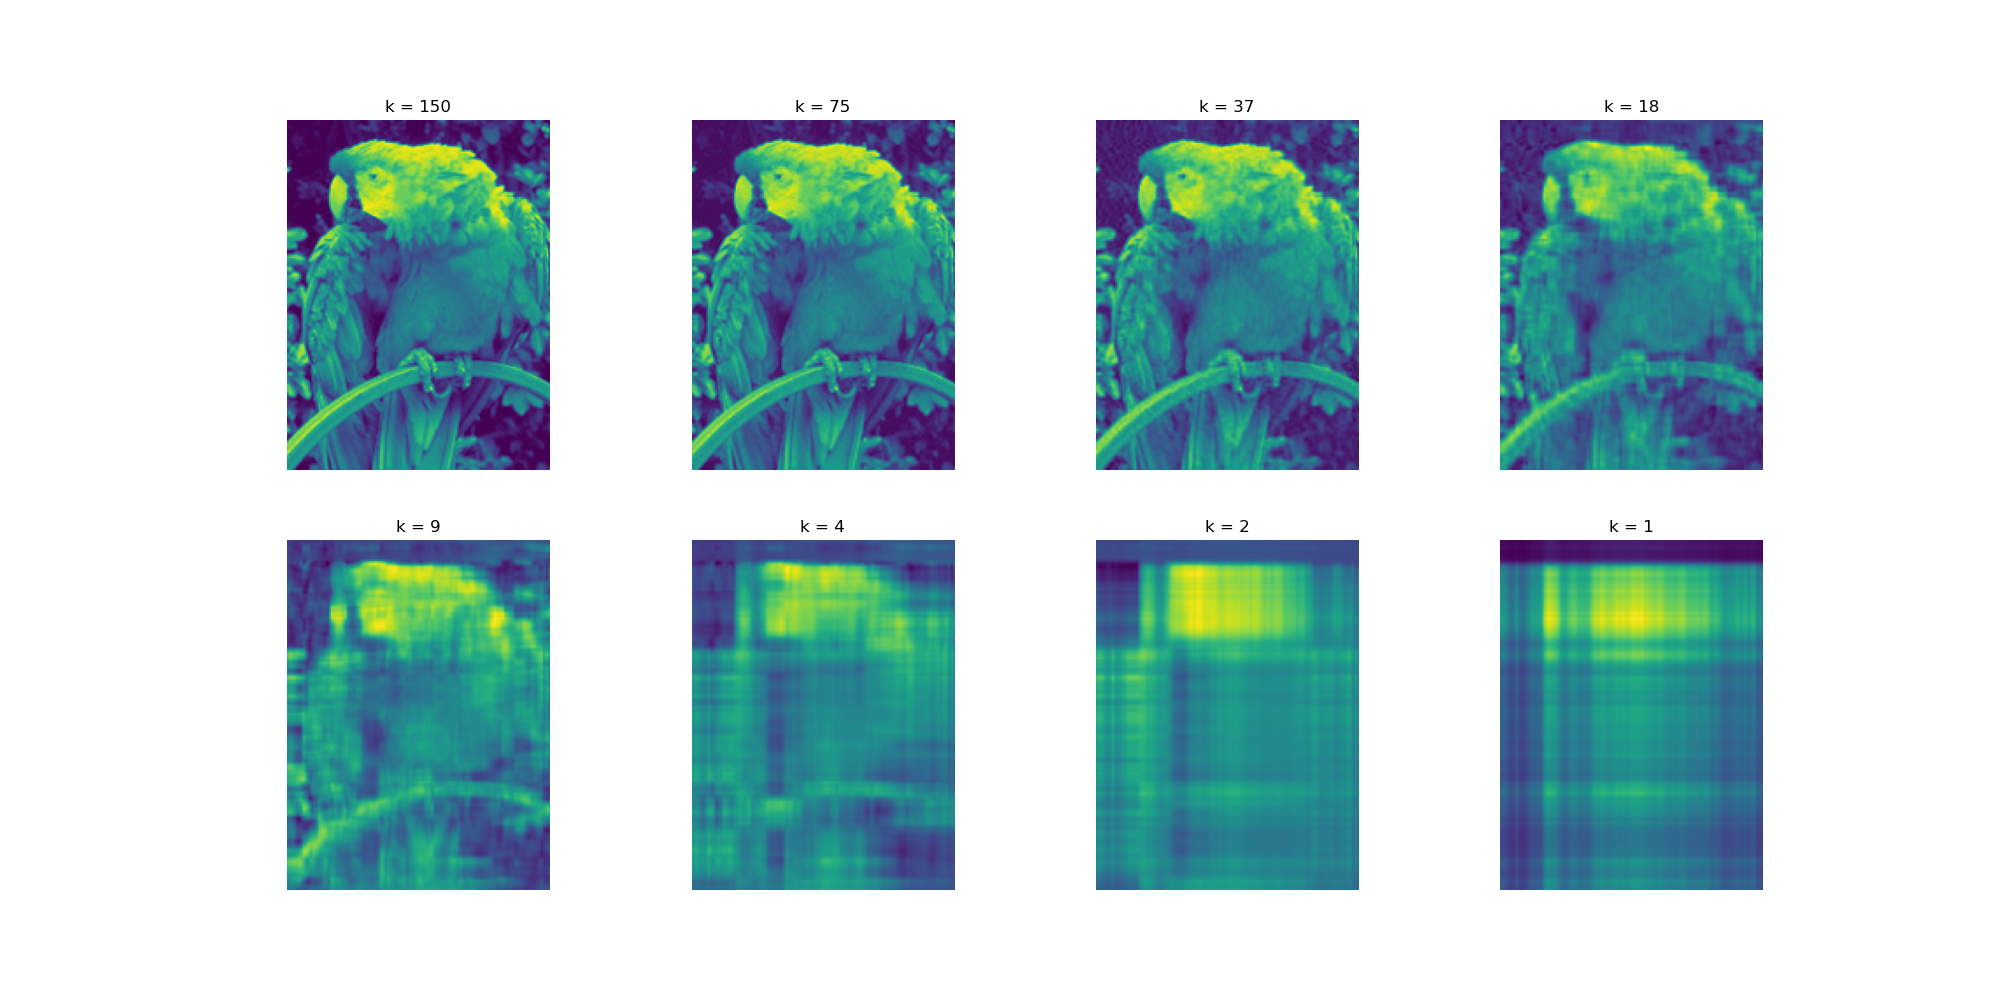
\includegraphics[width=\textwidth]{reconstructions_parrot.png}
\caption{Parrot image}
\end{figure}
In my opinion, k=10 does not degrade the image to badly. This corresponds to a reduction in storage space of 88.3\%.
% Inline Python code in the document
\begin{lstlisting}[language=Python]
# Updated dimensions for the original image
m = 200  # Height of the image
n = 150  # Width of the image
k = 10   # Rank for SVD compression

# Recalculate the storage requirements
storage_original = m * n
storage_compressed = k * (m + n + 1)

# Calculate the new savings
savings = 1 - (storage_compressed / storage_original)
savings_percentage = savings * 100  # Convert to percentage

storage_original, storage_compressed, savings_percentage
\end{lstlisting}
We also computed the Frobenius norm as a function of the rank $k$ for the parrot image. The results are shown in the plot below.
\begin{figure}
\centering
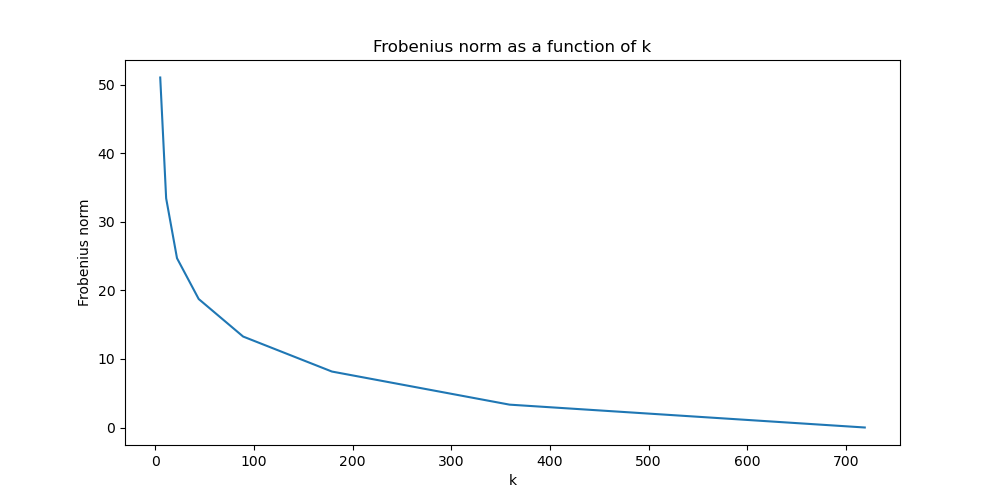
\includegraphics[width=\textwidth]{frobenius_norms.png}
\caption{Frobenius norms for the parrot image}
\end{figure}
The plot shows that the Frobenius norm decreases as the rank $k$ increases, which is expected. The Frobenius norm quantifies the difference between the original image and the compressed image, so a lower value indicates a better approximation. The plot also shows that the rate of decrease slows down as $k$ increases, which is also expected. This is because the largest singular values capture most of the information in the image, and the additional singular values contribute less to the overall image.
Another example:
\begin{figure}
\centering
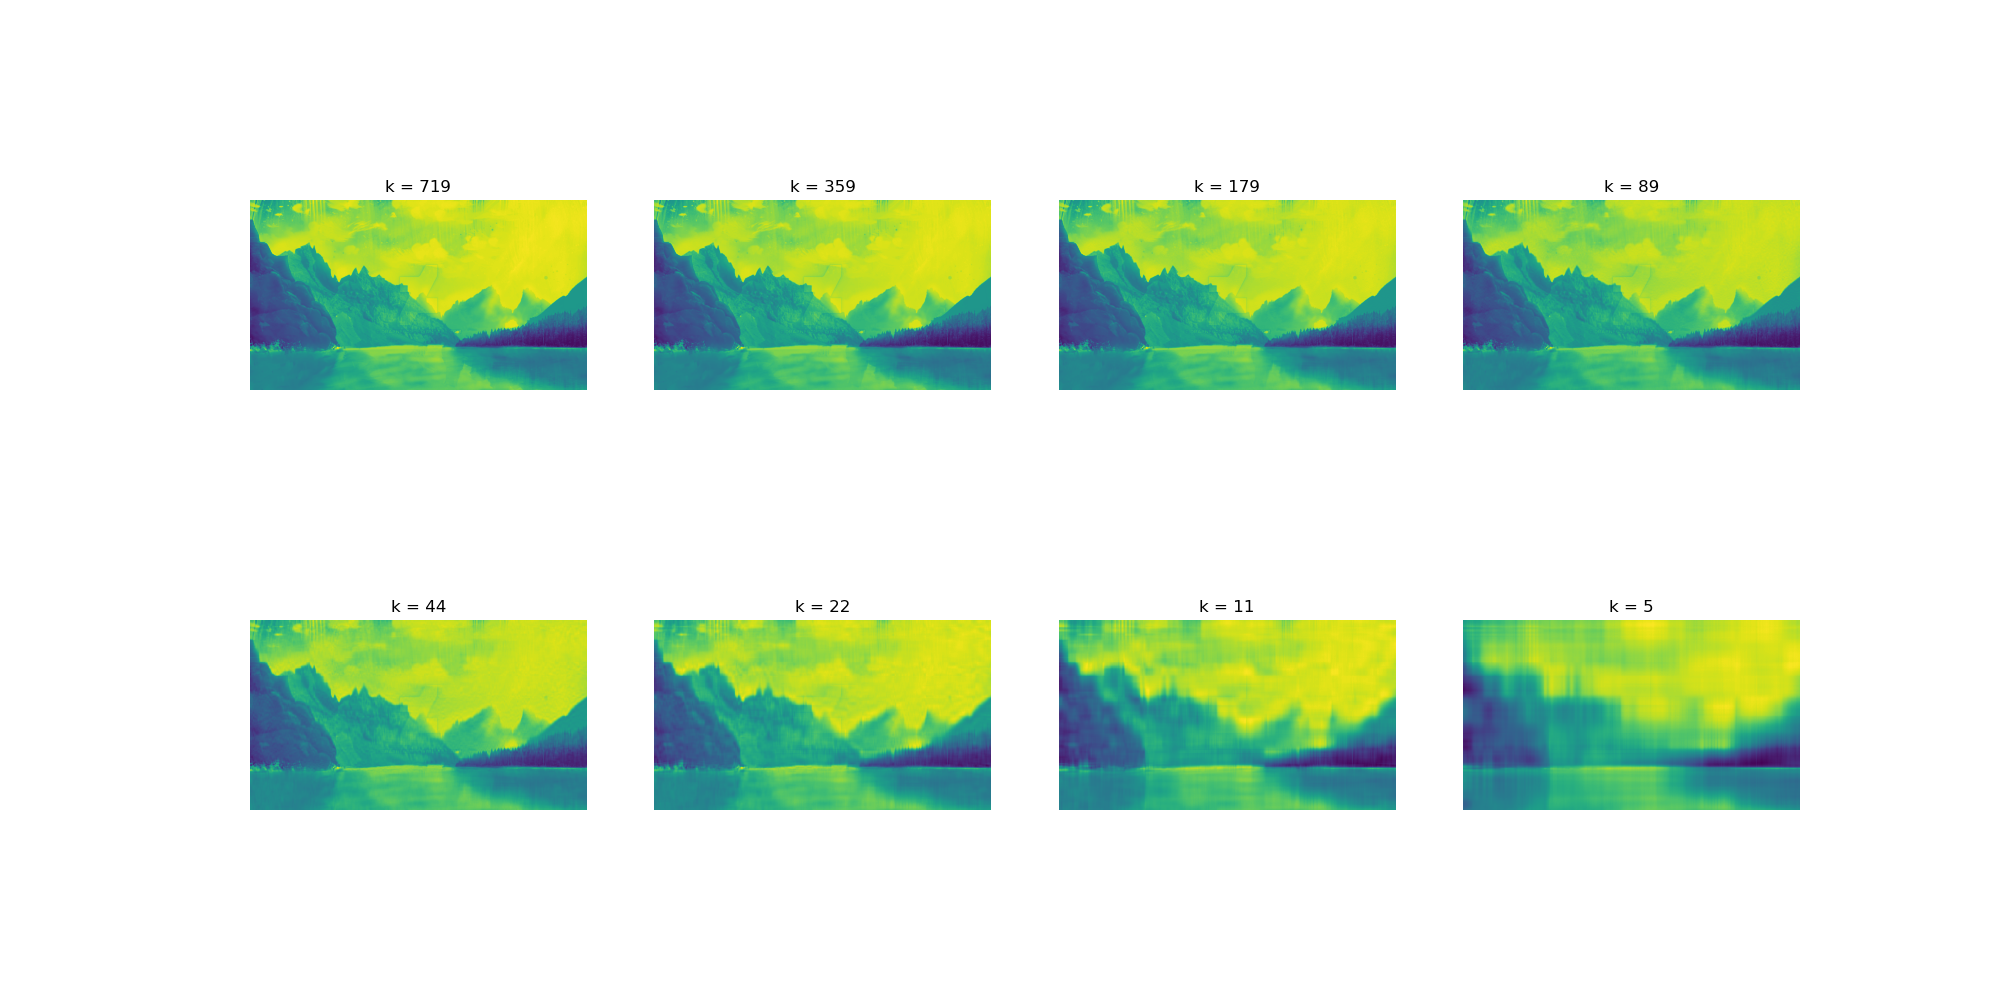
\includegraphics[width=\textwidth]{reconstructions_landscape.png}
\caption{Landscape image}
\end{figure}
\newpage
\subsection*{5.2 Entanglement entropy in ground states}
In the rest of this assignment, you will use eigenstates of the quantum Ising Hamiltonian found by your ED code from Assignment 1, and will calculate singular value spectra and entanglement\\
entropy (EE) for different subsystems, studying size dependence on $\ell$ and $L$. Use a sparse eigensolver for the ground state to reach larger system sizes.

Find the ground state of the quantum Ising chain for a fixed chain length $L$ and control parameter $h / J$; as in Assignment 1, solve at representative points in the ferromagnetic and paramagnetic phases and at the critical point. First impose open boundary conditions. Consider a segment $A$ of $\ell$ sites starting at the left end of the chain and calculate the entanglement entropy $S(\ell ; L)$ of this region. Plot $S(\ell ; L)$ for $1 \leq \ell \leq L-1$, and repeat this for several system sizes $L$; as a summary of these studies, plot also $S(L / 2, L)$ versus $L$.
\newpage
% Inline Python code in the document
\begin{lstlisting}[language=Python]
def entanglement_entropy(rho):
    """Calculate the entanglement entropy of a reduced density matrix."""
    # Normalize rho
    rho /= np.trace(rho)
    # Eigenvalues of the reduced density matrix
    eigvals = np.linalg.eigh(rho)[0]
    # Filter out zero eigenvalues to avoid log(0)
    nonzero_eigvals = eigvals[eigvals > 1e-10]
    # Entanglement entropy calculation
    entropy = -np.sum(nonzero_eigvals * np.log(nonzero_eigvals))
    return entropy

def calculate_reduced_density_matrix(state, L, ell):
    """Calculate the reduced density matrix for segment A of length ell."""
    # Reshape the state vector into a matrix
    state_matrix = state.reshape(2**ell, 2**(L - ell))
    # Calculate the reduced density matrix
    rho_A = np.dot(state_matrix, state_matrix.conj().T)
    return rho_A


L = [4, 6, 8]
h = [0.3, 1, 1.7]

entropies = {l: [] for l in L}
# Initialize data collection
S_L2_vs_L = {hi: [] for hi in h}  # This will hold entropy values for each h across all L


for l in L:
    for hi in h:
        # Calculate the ground state using the sparse_hamiltonian
        H = sparse_hamiltonian(l, hi, periodic=False)
        eigenvalues, eigenvectors = scipy.sparse.linalg.eigsh(H.astype(np.float64), k=1, which='SA')
        ground_state = eigenvectors[:, 0]
        
        for ell in range(1, l):
            rho_A = calculate_reduced_density_matrix(ground_state, l, ell)
            entropy = entanglement_entropy(rho_A)
            entropies[l].append(entropy)
        
        rho_A_L2 = calculate_reduced_density_matrix(ground_state, l, l//2)
        entropy_L2 = entanglement_entropy(rho_A_L2)
        S_L2_vs_L[hi].append((l, entropy_L2))  # Store the tuple (L, entropy)
# Define line styles for different values of h and colors for L
line_styles = ['-', '--', ':']
colors = ['b', 'g', 'r', 'c', 'm', 'y', 'k']  # Extend if needed
markers = ['o', '^', 's']  # Example: circle, triangle, square

if len(colors) < len(L):
    raise ValueError("Not enough colors for the number of L values")

# Plot S(ell; L) for 1 <= ell <= L-1 for various L and h
plt.figure(figsize=(10, 6))
for l_index, l in enumerate(L):
    color = colors[l_index]  # Color for each L
    for h_index, hi in enumerate(h):
        start_index = h_index * (l - 1)
        end_index = start_index + l - 1
        line_style = line_styles[h_index % len(line_styles)]
        plt.plot(range(1, l), entropies[l][start_index:end_index], label=f'L = {l}, h = {hi}',
                 linestyle=line_style, color=color)

plt.xlabel(r'Segment length $\ell$')
plt.ylabel(r'Entanglement Entropy $S(\ell; L)$')
plt.legend()
plt.title(r'Entanglement Entropy $S(\ell; L)$ vs. Segment length $\ell$')
plt.grid(True)
plt.savefig('entanglement_entropy.png')
\end{lstlisting}
I have attached both plots. The following interpretations can be made. It can be noticed that when the segment length is half of the system size, an equal cut of the full Hamiltonian is made, and this maximizes the entanglement entropy for the given system size; the entanglement entropy falls off when an uneven cut is made.
\begin{figure}
\centering
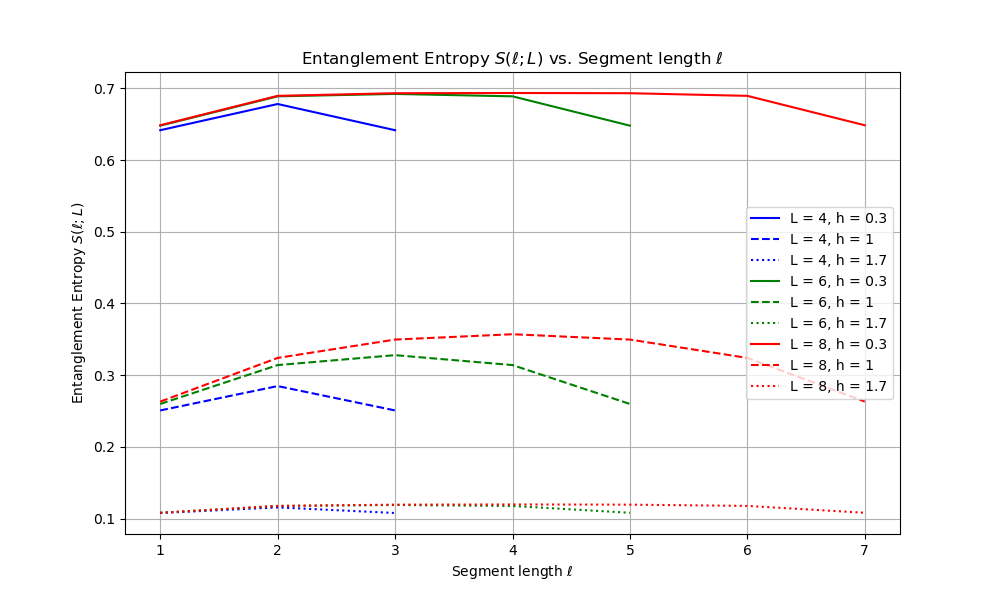
\includegraphics[width=\textwidth]{entanglement_entropy.png}
\caption{Entanglement entropy for different system sizes}
\end{figure}
\begin{figure}
\centering
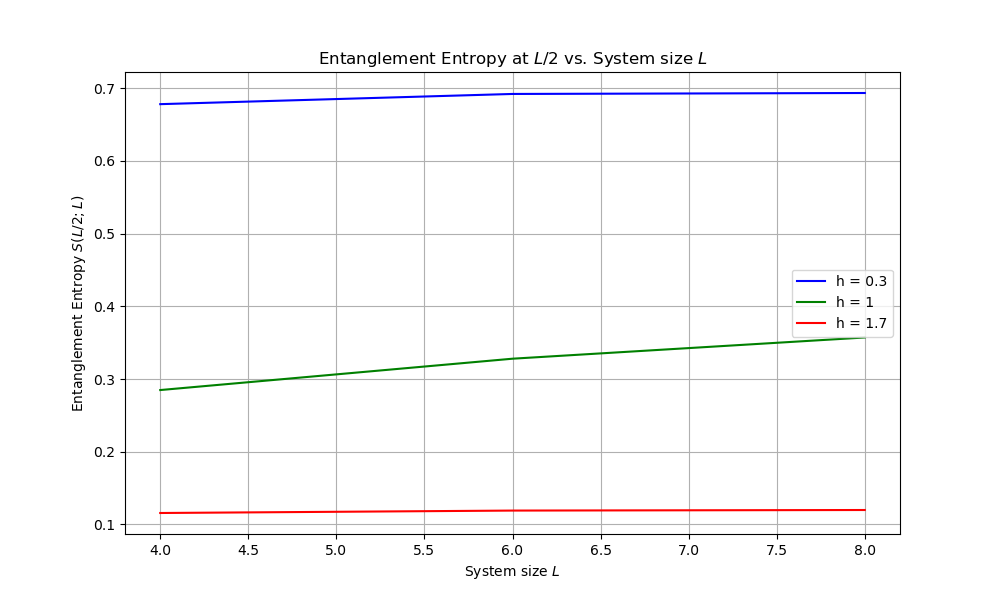
\includegraphics[width=\textwidth]{entanglement_entropy_L2.png}
\caption{Entanglement entropy at the midpoint of the chain as a function of system size}
\end{figure}
% Inline Python code in the document
\begin{lstlisting}[language=Python]
# Create the plot
plt.figure(figsize=(10, 6))
for h_index, hi in enumerate(h):
    color = colors[h_index % len(colors)]
    # Unpack L and entropy values for plotting
    L_vals, entropies = zip(*S_L2_vs_L[hi])
    plt.plot(L_vals, entropies, label=f'h = {hi}', color=color, linestyle='-')

plt.xlabel(r'System size $L$')
plt.ylabel(r'Entanglement Entropy $S(L/2; L)$')
plt.title(r'Entanglement Entropy at $L/2$ vs. System size $L$')
plt.legend()
plt.grid(True)
plt.savefig('entanglement_entropy_L2.png')
\end{lstlisting}
In the ferromagnetic phase, there are two possible ground states, so the entanglement entropy is near $\log 2 \approx 0.7$. In the paramagnetic phase, there is only one possible ground state, so the entanglement entropy is near $\log 1 \approx 0$. At the critical value for $h$, this is somewhere in the middle.
\newpage

Now consider the case with periodic boundary conditions and repeat the same calculations (the steps are identical to the open b.c. case). Why is the EE larger in the periodic case and roughly by what factor? \\\\
The area law tells us that the entanglement entropy will scale with the size of the boundary between the two regions. In the case of periodic boundary conditions, there can be 2 boundaries come as shown in the screenshot, while with open boundary conditions, there is only 1 boundary site in the middle of the chain. This is why the entanglement entropy is larger in the periodic case, roughly by a factor of 2.
\begin{figure}
\centering
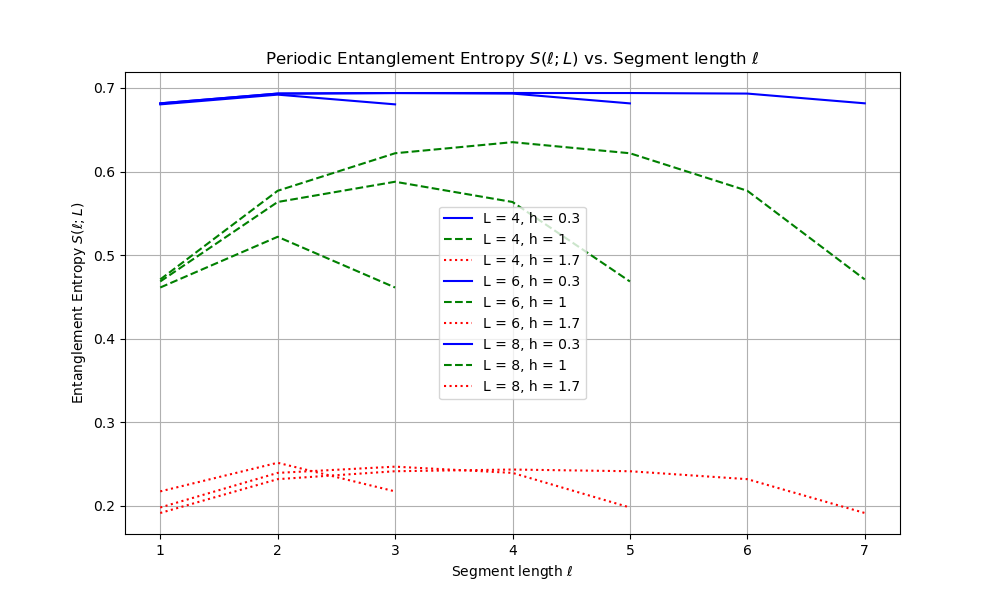
\includegraphics[width=\textwidth]{entanglement_entropy_periodic.png}
\caption{Entanglement entropy for different system sizes with periodic boundary conditions}
\end{figure}
For the periodic case, I just changed
% Inline Python code in the document
\begin{lstlisting}[language=Python]
H = sparse_hamiltonian(l, hi, periodic=True)  # Corrected to periodic=True as needed
\end{lstlisting}
\begin{figure}
\centering
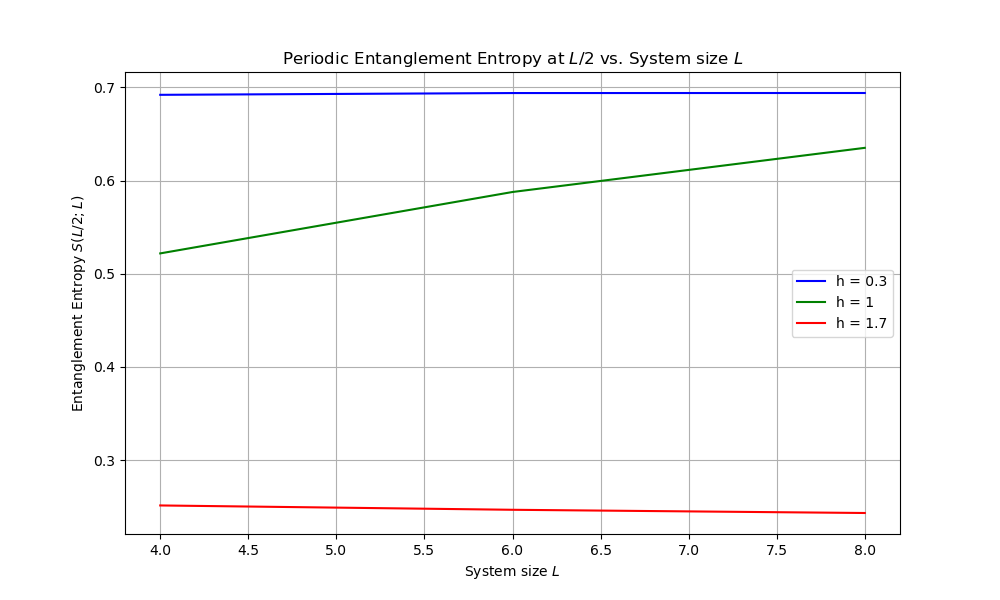
\includegraphics[width=\textwidth]{entanglement_entropy_L2_periodic.png}
\caption{Entanglement entropy at the midpoint of the chain as a function of system size with periodic boundary conditions}
\end{figure}
\begin{figure}
\centering
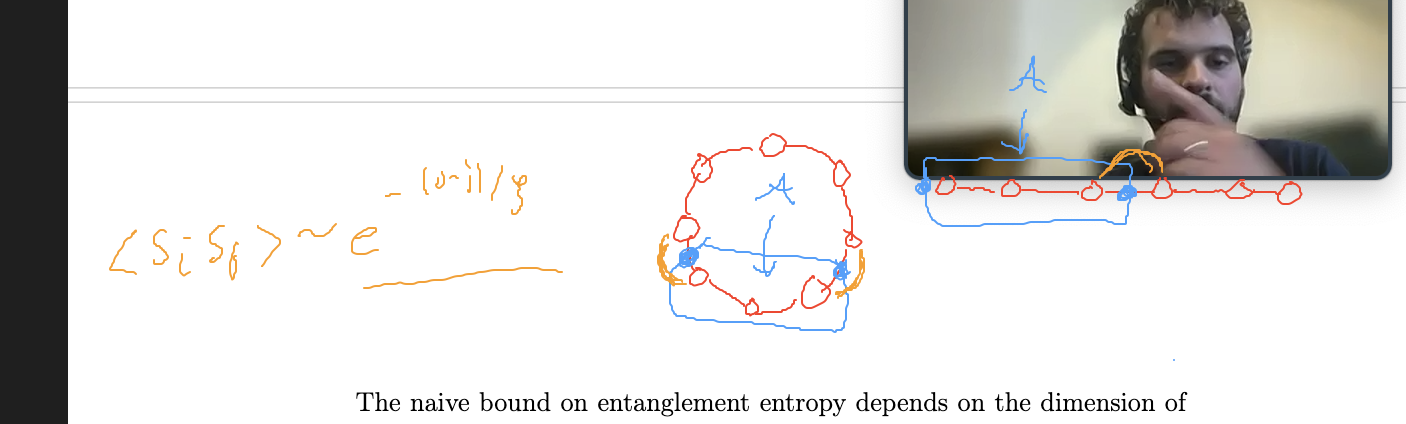
\includegraphics[width=\textwidth]{pbc.png}
\caption{Periodic vs. open boundary conditions}
\end{figure}
\newpage
For the largest system size, fit $S(\ell ; L)$ at the critical point to the following form:


\begin{equation*}
S(\ell ; L)=\frac{c}{3} \log \left(\frac{L}{\pi} \sin \frac{\pi \ell}{L}\right)+C \tag{26}
\end{equation*}


This form reduces to $S(\ell) \sim \frac{c}{3} \log \ell$ in the thermodynamic limit $(1 \ll \ell \ll L)$ but also nicely captures finite-size effects. (Remember to use the same log base when defining the entanglement entropy and when fitting this form.)\\\\
I did a fit for this at the critical point and L=8.
% Inline Python code in the document
\begin{lstlisting}[language=Python]
# Correct the definition of the fit function
def fit_function(ell, c, C):
    # Assuming max(L) is the largest value in your L array
    largest_L = max(L)  
    return (c / 3) * np.log((largest_L / np.pi) * np.sin(np.pi * ell / largest_L)) + C

# Correct the extraction of critical data
# This assumes that entropies[max(L)] contains the entropies for the largest system size at the critical point h=1
critical_ell = np.array(range(1, max(L)))  # This should generate 8 values if max(L) is 8
critical_ee = np.array(entropies[max(L)])  # Make sure this has the same number of values as critical_ell


# Fit the data to the equation
params, params_covariance = curve_fit(fit_function, critical_ell, critical_ee)

# Plot the fit results
plt.figure()
plt.plot(critical_ell, critical_ee, 'bo', label='Data')
plt.plot(critical_ell, fit_function(critical_ell, *params), 'r-', label=f'Fit: ${params[0]:.2f}/3 \log((L/\pi) \sin(\pi \ell / L)) + {params[1]:.2f}$')
plt.xlabel(r'Segment length $\ell$')
plt.ylabel(r'Entanglement Entropy $S(\ell; L)$')
plt.legend()
plt.title('Fit of Entanglement Entropy at Critical Point')
plt.grid(True)
plt.savefig('entanglement_entropy_fit.png')

# Output the fit parameters
print(f"Fitted c: {params[0]}")
print(f"Fitted C: {params[1]}")


\end{lstlisting}
\begin{figure}
\centering
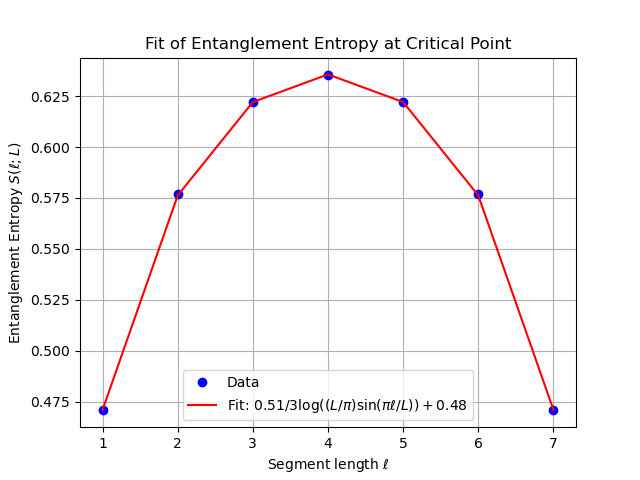
\includegraphics[width=\textwidth]{entanglement_entropy_fit.png}
\caption{Fit of the entanglement entropy at the critical point}
\end{figure}
\newpage

Have your eigensolver find the highest excited state of the Hamiltonian and perform a similar study; here it is enough to consider just one value of $h / J \neq(h / J)_{c}$ and one choice of boundary conditions. Why do you think the highest-energy state also satisfies the area law?\\\\
I did the same thing for the highest excited state but with the open boundary conditions. 
\begin{figure}
\centering
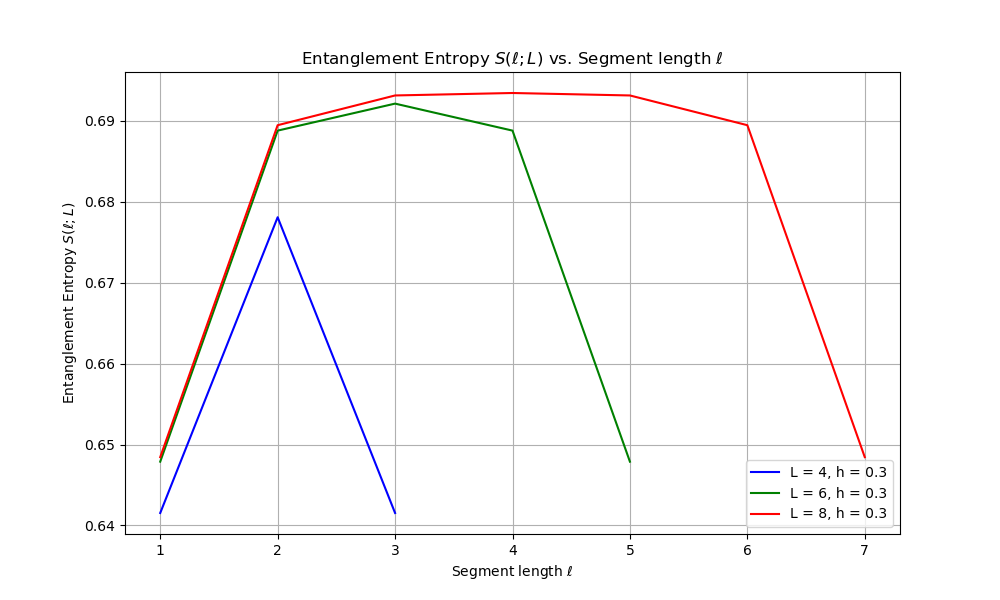
\includegraphics[width=\textwidth]{entanglement_entropy_LA.png}
\caption{Entanglement entropy for the highest excited state}
\end{figure}

\begin{figure}
\centering
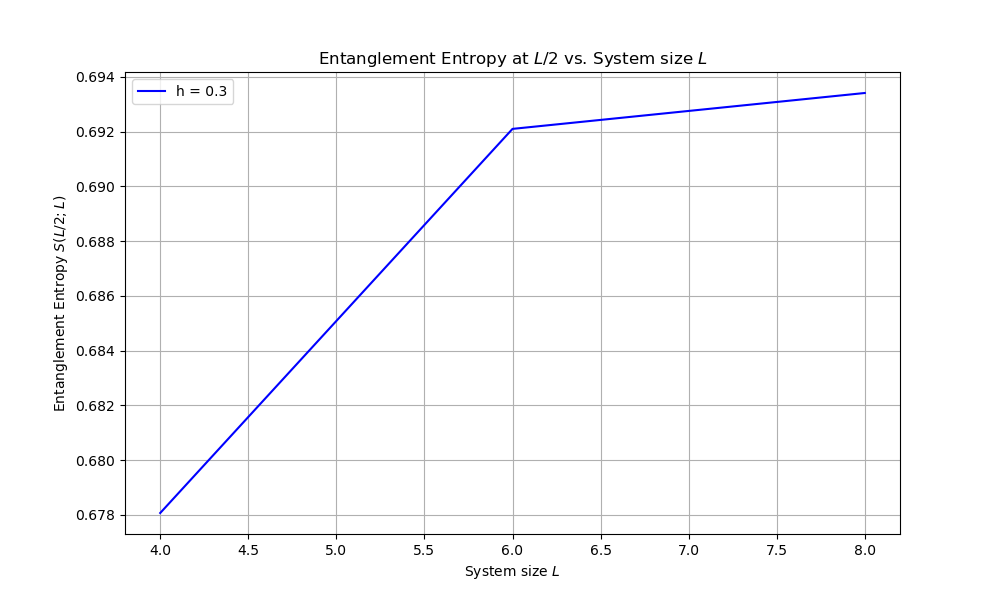
\includegraphics[width=\textwidth]{entanglement_entropy_L2_LA.png}
\caption{Entanglement entropy at the midpoint of the chain for the highest excited state}
\end{figure}
% Inline Python code in the document
\begin{lstlisting}[language=Python]
eigenvalues, eigenvectors = scipy.sparse.linalg.eigsh(H.astype(np.float64), k=1, which='LA')
\end{lstlisting}
\newpage

\subsection*{5.3 Truncation error of Schmidt decomposition}
Consider again the Ising ground state at representative values of the control parameter $h / J$, using open boundary conditions. Perform the Schmidt decomposition at the middle of the chain and compute the approximate ground state arising from truncating the factorization at $k$ ranging from 1 to $2^{L / 2}$. For each $k$, calculate the discarded norm (Frobenius error) $d(k)$, as well as the error in energy of the approximate ground state, using $E=\langle\psi|H| \psi\rangle /\langle\psi \mid \psi\rangle$. Plot $\Delta E(k)$ as a function of $d(k)$; you should find a roughly linear relationship. This technique is used in MPS methods to extrapolate exact ground state energy to the $k \rightarrow \infty$ limit, using only low- $k$ data.
\begin{figure}
\centering
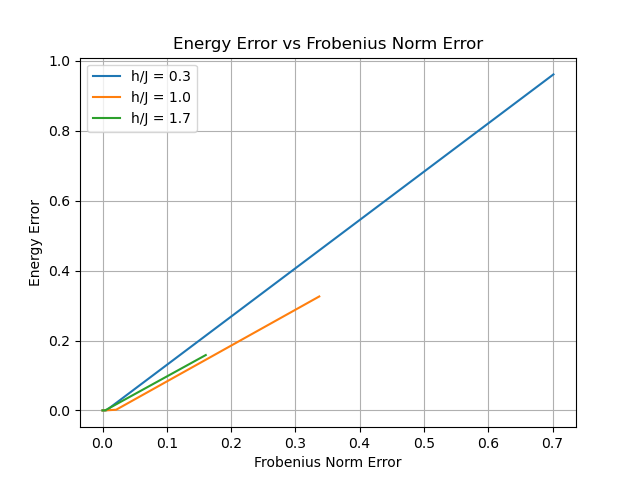
\includegraphics[width=\textwidth]{energy_vs_frobenius.png}
\caption{Truncation error of the Schmidt decomposition}
\end{figure}
% Inline Python code in the document
\begin{lstlisting}[language=Python]
from hw1 import sparse_hamiltonian
import numpy as np
import matplotlib.pyplot as plt

def schmidt_decomposition(psi, L):
    """Performs Schmidt decomposition at the middle of the chain."""
    cut_psi = psi.reshape(2**(L//2), -1)
    U, s, Vt = np.linalg.svd(cut_psi, full_matrices=False)
    return cut_psi, U, s, Vt

def truncated_state(U, S, Vh, k):
    """Reconstructs the state using only the first k singular values."""
    Sk = np.zeros_like(S)
    Sk[:k] = S[:k]
    flat_psi_k = U @ np.diag(Sk) @ Vh
    return flat_psi_k, flat_psi_k.flatten()

h_values = [0.3, 1, 1.7]
L = 8
errors = {hi: [] for hi in h_values}

# Single loop to handle everything per each h
for hi in h_values:
    # Compute the ground state
    H = sparse_hamiltonian(L, hi, periodic=False)
    eigenvalues, eigenvectors = np.linalg.eigh(H.toarray())
    ground_state = eigenvectors[:, 0]
    
    # Perform Schmidt decomposition
    original, U, s, Vt = schmidt_decomposition(ground_state, L)
    
    # Loop through all possible k values for truncation
    for k in range(1, 2**(L//2) + 1):
        mat_psi_k, flat_psi_k = truncated_state(U, s, Vt, k)
        norm_error = np.linalg.norm(original - mat_psi_k, 'fro')
        psi_k_energy = (flat_psi_k.conj().T @ H @ flat_psi_k) / (flat_psi_k.conj().T @ flat_psi_k)
        energy_error = np.abs(psi_k_energy - eigenvalues[0])
        errors[hi].append((norm_error, energy_error))

# Plotting the results
for hi, error_list in errors.items():
    norm_errors, energy_errors = zip(*error_list)
    plt.plot(norm_errors, energy_errors, label=f'h/J = {hi:.1f}')

plt.xlabel('Frobenius Norm Error')
plt.ylabel('Energy Error')
plt.title('Energy Error vs Frobenius Norm Error')
plt.legend()
plt.grid()
plt.savefig('energy_vs_frobenius.png')
\end{lstlisting}
\newpage

\subsection*{5.4 Entanglement entropy of highly excited states}
Now we will calculate the entanglement entropy $S(\ell; L)$ for an eigenstate in the middle of the many-body spectrum. Here, consider just one value of $h/J$ (e.g., in the paramagnetic phase) and one choice of boundary conditions (e.g., periodic b.c.), but perform a systematic study of $S(\ell, L)$ for several $L$. Note that the sparse eigensolver does not work in the middle of the spectrum, so you will need a full diagonalization and will thus access smaller systems. To avoid complications with resolving degeneracies, consider a few eigenstates corresponding to non-degenerate eigenvalues close to zero energy (which is exactly in the middle of the spectrum in this model). You will see that the entanglement entropy is much larger for states in the middle of the spectrum compared to the band edges and should observe volume law scaling on average.\\
\begin{figure}[h]
\centering
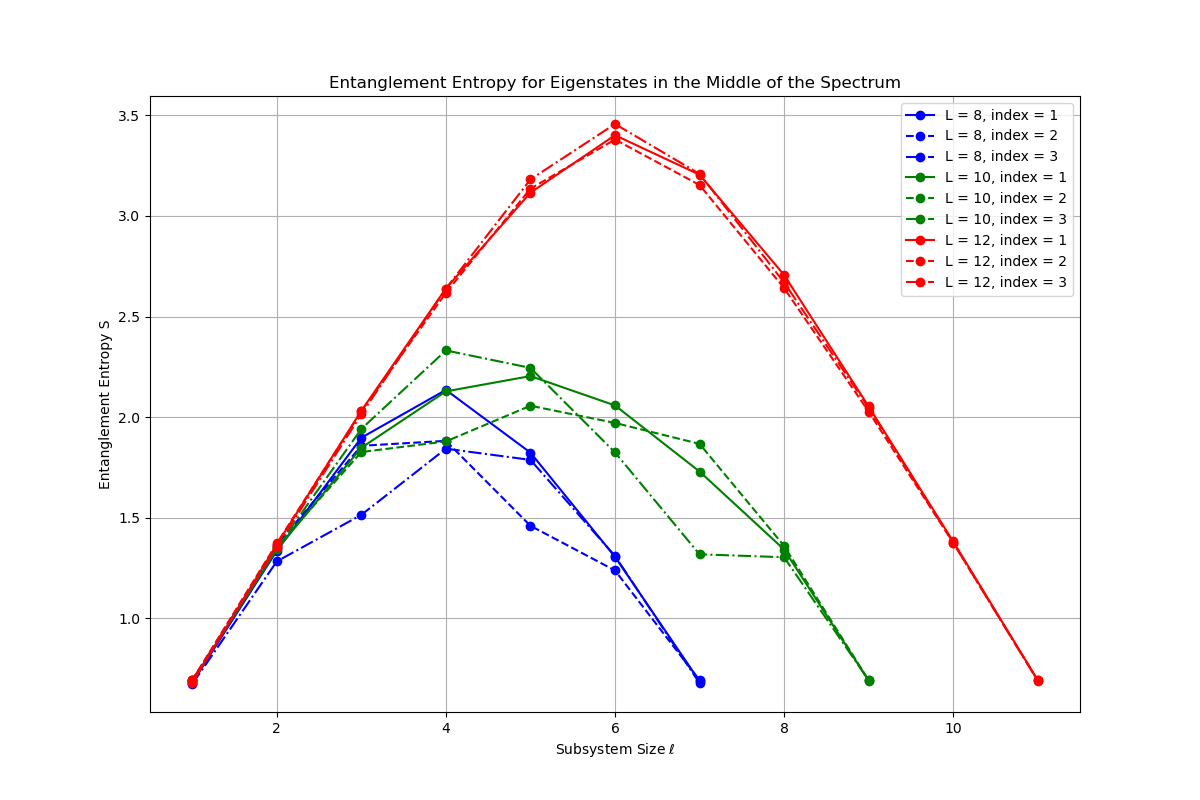
\includegraphics[width=\textwidth]{entanglement_entropy_middle_spectrum.png}
\caption{Entanglement entropy for eigenstates in the middle of the spectrum}
\end{figure}
What can be observed here is that the entanglement entropy for ground states ranged from 0.3-0.7, but in this case, it can range from like 1.0-3.5 for the states in the middle of the spectrum. This is a result of there being more excited states with the same eigenvalue to choose from than just the ground state. For the ferromagnetic phase that we are considering here, there were 2 ground states to choose from so the entanglement entropy was bounded by $\log 2 \approx 0.7$. Also, we see a manifestation of the volume law, where the larger system sizes show a larger entanglement entropy.
% Inline Python code in the document
\begin{lstlisting}[language=Python]
from hw1 import periodic_dense_hamiltonian_explicit
from p5_2 import entanglement_entropy, calculate_reduced_density_matrix
import numpy as np
import matplotlib.pyplot as plt

h = 1.7
L_sizes = [6, 8, 10, 12]  # Different system sizes
entropies = {L: [] for L in L_sizes}  # Dictionary to store entropies by L

for L in L_sizes:
    H = periodic_dense_hamiltonian_explicit(L, h)
    eigenvalues, eigenvectors = np.linalg.eigh(H)

    # Select a eigenstate near the middle of the spectrum
    mid_index = len(eigenvalues) // 2
    # make sure that it is not degenerate
    if eigenvalues[mid_index] != eigenvalues[mid_index + 1] and eigenvalues[mid_index] != eigenvalues[mid_index - 1]:
        state = eigenvectors[:, mid_index]
    else:
        # If the middle index is degenerate, shift slightly to find a non-degenerate state
        offset = 1
        while (mid_index + offset < len(eigenvalues) and eigenvalues[mid_index] == eigenvalues[mid_index + offset]) or \
              (mid_index - offset >= 0 and eigenvalues[mid_index] == eigenvalues[mid_index - offset]):
            offset += 1
        state = eigenvectors[:, mid_index + offset]

    # Compute the entanglement entropy for each ell using the same procedure as in p5_2.py
    for ell in range(1, L):
        rho_A = calculate_reduced_density_matrix(state, L, ell)
        entropy = entanglement_entropy(rho_A)
        entropies[L].append((ell, entropy))  # Store ell and entropy

# Plotting the results
plt.figure(figsize=(10, 6))
for L in L_sizes:
    ells, L_entropies = zip(*entropies[L])  # Unpack ell and entropy values for each L
    plt.plot(ells, L_entropies, marker='o', linestyle='-', label=f'L = {L}')

plt.xlabel('Subsystem Size ell')
plt.ylabel('Entanglement Entropy S')
plt.title('Entanglement Entropy for Eigenstates in the Middle of the Spectrum')
plt.legend()
plt.grid(True)
plt.savefig('entanglement_entropy_middle_spectrum.png')
\end{lstlisting}
\newpage
\subsection*{5.4.1 Optional. Volume law for random states}
Generate a random vector in the same Hilbert space of $L$ spins and study its entanglement $S(\ell ; L)$. You will get a reasonably random vector by simply choosing an i.i.d. random value - for example, uniformly distributed in $[-1,1]$ - for each amplitude of the $2^{L}$ basis states. However, in order\\
to actually sample a random vector with a basis-independent distribution uniform over the unit sphere (in the manifold of states that can be written as real-valued wavefunctions), you can choose coefficients from a Gaussian distribution. Remember to normalize your vectors. Repeating this process, you will observe average scaling with the volume law of entanglement.
\newpage

\subsection*{5.5 Matrix product state representation for ground states}
Return to the setup in Sec. 5.2, considering the ground state $\left|\psi_{\text {gs }}\right\rangle$ with open b.c., using a sparse eigensolver to reach larger sizes. You should now consider two points, one fairly close to the phase transition, say $h / J=5 / 4$, and one exactly at $h / J=(h / J)_{c}=1$. Compute MPS approximations of the ED wavefunction, varying the bond dimension $k$. What is the actual reduction in storage space you achieve? Contract the virtual indices of the tensors of the MPS to obtain exponentially large $\left|\tilde{\psi}_{\mathrm{gs}}(k)\right\rangle$ and compute the overlap $\left\langle\tilde{\psi}_{\mathrm{gs}}(k) \mid \psi_{\mathrm{gs}}\right\rangle$ with the original ED wavefunction.
\subsubsection{Answer}
My results are shown. The approximation is not that good for k=1, but it is surprisingly good for the ground state as k increases even in small increments. This is likely because we tried to approximate the ground state which does not have much entanglement and can be well approximated as a product state. It also should be noted that the rank 2 approximation is so good because we are dealing with a system of 2 possible spins i.e. no more than 2 singular values are needed for a good approximation to the state.
\begin{figure}[h]
\centering
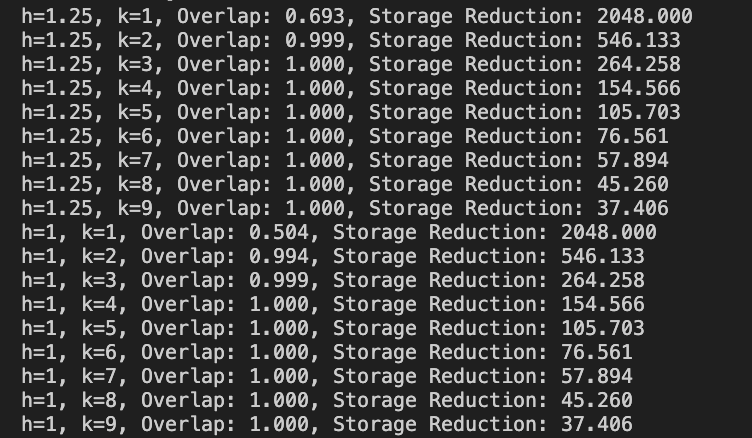
\includegraphics[width=\textwidth]{overlap.png}
\caption{Overlap between the MPS approximation and the exact ground state}
\end{figure}
% Inline Python code in the document
\begin{lstlisting}[language=Python]
import numpy as np
from scipy.sparse.linalg import eigsh  # Sparse matrix eigensolver
from hw1 import sparse_hamiltonian  # Assuming this function generates your Hamiltonian
from numpy.linalg import norm

def truncate_svd(matrix, k):
    """
    Truncates the singular value decomposition (SVD) of a matrix.

    Parameters:
    matrix (ndarray): The input matrix.
    k (int): The number of singular values to keep.

    Returns:
    ndarray: The truncated left singular vectors.
    ndarray: The truncated singular values.
    ndarray: The truncated right singular vectors.
    """
    u, s, vt = np.linalg.svd(matrix, full_matrices=False)
    return u[:, :k], np.diag(s[:k]), vt[:k, :]



def compute_mps(state, k):
    # this is just the length of the system
    L = int(np.log2(state.size))
    # prepare the state for the initial SVD
    state = state.reshape((2, -1))
    # list to store the mps tensors
    mps_tensors = []
    # initialize a previous bond dimension
    previous_k = 2

    # loop over the system
    for i in range(1, L+1):
        # make the SVD
        u, s, vt = truncate_svd(state, k)
        # current bond dimension
        current_k = min(k, u.shape[1])
        # debugging
        print(f'Current state shape: {state.shape}, u shape: {u.shape}, s shape: {s.shape}, vt shape: {vt.shape}')

        # for the first iteration
        if i == 1:
            mps_tensors.append(u.reshape((previous_k, -1)))
        # for the middle iterations
        elif i < L:
            # append the rank 3 tensor following the notation of the tensor network diagrams
            mps_tensors.append(u.reshape((previous_k, 2, current_k)))
        # for the last iteration
        else:
            mps_tensors.append(u.reshape((previous_k, -1)))
            break
        # prepare the state for the next iteration
        state = (s @ vt).reshape((2*current_k, -1))
        # update the previous bond dimension
        previous_k = current_k

    return mps_tensors





def reconstruct_state(mps_tensors):
    state = mps_tensors[0]  # Start with the first tensor, assumed to be a matrix.

    for j in range(1, len(mps_tensors)):
        next_tensor = mps_tensors[j]

        # this is for the first construction
        if len(state.shape) == 2:
            # print(f"before state shape: {state.shape}, tensor shape: {next_tensor.shape}")
            state = np.einsum('ij,jkl->ikl', state, next_tensor)
        # this is for the middle cases
        elif len(state.shape) == 3 and len(next_tensor.shape) == 3:
            state = state.reshape(-1, state.shape[2])
            # print(f"before state shape: {state.shape}, tensor shape: {next_tensor.shape}")
            state = np.einsum('ij,jkl->ikl', state, next_tensor)
        # now for the final case
        elif len(next_tensor.shape) == 2:
            state = state.reshape(-1, state.shape[2])
            next_tensor = next_tensor.reshape(state.shape[1], -1)
            print(f"before state shape: {state.shape}, tensor shape: {next_tensor.shape}")
            state = np.einsum('ij,jk->ik', state, next_tensor)
            

    return state.reshape(-1)  # Flatten the final state to a 1D array







def calculate_overlap(original, reconstructed):
    return np.abs(np.vdot(original, reconstructed) / (norm(original) * norm(reconstructed)))

# Parameters
L = 16 # System size
h_values = [5/4, 1]  # Near and at the critical point
k_values = np.arange(1, 10, 1)  # Bond dimensions for MPS, from 1 to 20 inclusive


results = {}

for h in h_values:
    H = sparse_hamiltonian(L, h, periodic=False)
    eigenvalues, eigenvectors = eigsh(H.astype(np.float64), k=1, which='SA')
    gs = eigenvectors[:, 0]
    gs /= np.linalg.norm(gs)
    results[h] = {}

    for k in k_values:
        mps_tensors = compute_mps(gs, k)
        print(mps_tensors)
        reconstructed_gs = reconstruct_state(mps_tensors)
        # print out the gs and reconstructed_gs
        print(f"gs: {gs}")
        print(f"reconstructed_gs: {reconstructed_gs}")
        overlap = calculate_overlap(gs, reconstructed_gs)
        num_params_original = gs.size
        num_params_mps = sum(t.size for t in mps_tensors)
        storage_reduction = num_params_original / num_params_mps
        results[h][k] = {
            'ground_state': gs,
            'mps': mps_tensors,
            'overlap': overlap,
            'storage_reduction': storage_reduction
        }

# Printing or processing results as needed
for h in results:
    for k in results[h]:
        print(f"h={h}, k={k}, Overlap: {results[h][k]['overlap']:.3f}, Storage Reduction: {results[h][k]['storage_reduction']:.3f}")

\end{lstlisting}
\newpage

\subsection*{5.5. Efficient calculations with MPS}
We will now make use of the efficient measurements afforded by MPS, which are described in Sec. 4.3. Set up such a calculation for $E(k)=\left\langle\tilde{\psi}_{\mathrm{gs}}(k)|H| \tilde{\psi}_{\mathrm{gs}}(k)\right\rangle /\left\langle\tilde{\psi}_{\mathrm{gs}}(k) \mid \tilde{\psi}_{\mathrm{gs}}(k)\right\rangle$ using the MPS, comparing your answer with the known energy eigenvalue that was given by your exact diagonalization routine. Also compute the same correlation functions you studied in Assignment 1, for both values of $h / J$, and examine the convergence of the results in each case for several values of $k$.
\subsubsection{Answer}
We know that the quantum Ising model has a Hamiltonian given by
\begin{equation*}
H=-J \sum_{i=1}^{L-1} \sigma_{i}^{z} \sigma_{i+1}^{z}-h \sum_{i=1}^{L} \sigma_{i}^{x} \tag{1}
\end{equation*}
where $\sigma_{i}^{x}, \sigma_{i}^{z}$ are the Pauli matrices acting on site $i$, and $J, h$ are the coupling constants. The ground state energy of the quantum Ising model can be calculated using the MPS representation of the ground state. The energy of the ground state is given by

\subsection*{5.5.2 Bringing an MPS to a canonical form with an orthogonality center}
Consider an MPS state of the form Eq. (19) with bond dimension 2 and matrices


\begin{align*}
& A^{(1) \uparrow}=\frac{1}{\sqrt{2}}\left(\begin{array}{ll}
1 & 1
\end{array}\right), \quad A^{(1) \downarrow}=\frac{1}{\sqrt{2}}\left(\begin{array}{ll}
1 & -1
\end{array}\right),  \tag{27}\\
& A^{(\ell) \uparrow}=\frac{1}{\sqrt{2}}\left(\begin{array}{ll}
1 & 1 \\
0 & 0
\end{array}\right), \quad A^{(\ell) \downarrow}=\frac{1}{\sqrt{2}}\left(\begin{array}{cc}
0 & 0 \\
1 & -1
\end{array}\right), \quad 2 \leq \ell \leq L-1,  \tag{28}\\
& A^{(L) \uparrow}=\left(\begin{array}{l}
1 \\
0
\end{array}\right), \quad A^{(L) \downarrow}=\left(\begin{array}{l}
0 \\
1
\end{array}\right) . \tag{29}
\end{align*}


(Aside note: this state is related to so-called cluster state in quantum information theory.) You can verify analytically that this is a very special state where at each $\ell=2, \ldots, L-1$ the matrices $A^{(\ell) \sigma}$ satisfy both left- and right-canonicity condition, while $A^{(1) \sigma}$ satisfy the left-canonicity and $A^{(L) \sigma}$ satisfy the right-canonicity. \\
Given the MPS matrices:
\[
A^{(1) \uparrow} = \frac{1}{\sqrt{2}}
\begin{bmatrix}
1 & 1
\end{bmatrix}, \quad
A^{(1) \downarrow} = \frac{1}{\sqrt{2}}
\begin{bmatrix}
1 & -1
\end{bmatrix}
\]

We compute the left-canonical condition:
\[
\left(A^{(1) \uparrow}\right)^\dagger A^{(1) \uparrow} + \left(A^{(1) \downarrow}\right)^\dagger A^{(1) \downarrow}
\]

Calculating each term:
\[
\left(A^{(1) \uparrow}\right)^\dagger = \frac{1}{\sqrt{2}}
\begin{bmatrix}
1 \\
1
\end{bmatrix}, \quad
\left(A^{(1) \downarrow}\right)^\dagger = \frac{1}{\sqrt{2}}
\begin{bmatrix}
1 \\
-1
\end{bmatrix}
\]

\[
\left(A^{(1) \uparrow}\right)^\dagger A^{(1) \uparrow} = \frac{1}{2}
\begin{bmatrix}
1 & 1 \\
1 & 1
\end{bmatrix}, \quad
\left(A^{(1) \downarrow}\right)^\dagger A^{(1) \downarrow} = \frac{1}{2}
\begin{bmatrix}
1 & -1 \\
-1 & 1
\end{bmatrix}
\]

Summing these:
\[
\frac{1}{2}
\begin{bmatrix}
1 & 1 \\
1 & 1
\end{bmatrix} + \frac{1}{2}
\begin{bmatrix}
1 & -1 \\
-1 & 1
\end{bmatrix} = 
\begin{bmatrix}
1 & 0 \\
0 & 1
\end{bmatrix}
\]

This shows that the sum is the identity matrix, satisfying the left-canonical condition. Proving the right canonical condition will be similar. ChatGPT was also able to convince me that the middle matrices satisfy both the left and right canonicity conditions.\\
Hence, this state can be viewed also as being in the canonical form whose orthogonality center can be viewed as located anywhere along the chain. What are the Schmidt values across any cut? (Hint: matrix $S$ is not explicitly present but what such matrix can you trivially insert? The state is not normalized but the normalization can be trivally achieved.) \\\\
You can trivially insert the identity matrix.\\\\
For some reasonable $L$, have the computer write out the full wavefunction in the computational basis by multiplying out the matrices. By reusing your previous routines, verify the analytical predictions for the Schmidt values across any cut.
\newpage
I did this and I verified that the Schmidt values across any cut are 1.
\begin{figure}[h]
\centering
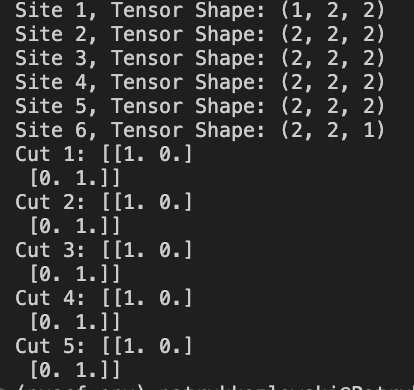
\includegraphics[width=\textwidth]{schmidt1.png}
\caption{Schmidt values across any cut}
\end{figure}
% Inline Python code in the document
\begin{lstlisting}[language=Python]
import numpy as np
from p5_5 import truncate_svd

# Define MPS matrices for a chain
L = 6  # Number of sites
mps_tensors = []

# Initial tensor setup
A_1_up = np.array([1, 1]) / np.sqrt(2)
A_1_down = np.array([1, -1]) / np.sqrt(2)
mps_tensors.append(np.stack((A_1_up, A_1_down), axis=0).reshape(1, 2, 2))  # First tensor

# # initial tensor setup for second part
# A_1_up = np.array([1, 2])
# A_1_down = np.array([2, -1])
# mps_tensors.append(np.stack((A_1_up, A_1_down), axis=0).reshape(1, 2, 2))  # First tensor

# Middle tensors
for site in range(1, L-1):
    A_ell_up = np.array([[1, 1], [0, 0]]) / np.sqrt(2)
    A_ell_down = np.array([[0, 0], [1, -1]]) / np.sqrt(2)
    mps_tensors.append(np.stack((A_ell_up, A_ell_down), axis=0))

# Last tensor
A_L_up = np.array([1, 0])
A_L_down = np.array([0, 1])
mps_tensors.append(np.stack((A_L_up, A_L_down), axis=0).reshape(2, 2, 1))  # Last tensor

# # last tensor for second part
# A_L_up = np.array([1, 3])
# A_L_down = np.array([3, 1])
# mps_tensors.append(np.stack((A_L_up, A_L_down), axis=0).reshape(2, 2, 1))  # Last tensor


# Display tensor shapes
for idx, tensor in enumerate(mps_tensors):
    print(f"Site {idx+1}, Tensor Shape: {tensor.shape}")

# Calculate Schmidt values at each cut
for cut in range(1, L):
    # Contract tensors to the left of the cut
    left_state = mps_tensors[0].reshape(-1, 2)  # Start with the first tensor reshaped for matrix multiplication
    # first make a loop from 1 to cut - 1
    for i in range(1, cut):
        left_state = np.einsum('ab,bcd->acd', left_state, mps_tensors[i])
        left_state = left_state.reshape(-1, mps_tensors[i].shape[2])  # Ensure correct shape

    # Contract tensors to the right of the cut
    right_state = mps_tensors[cut].reshape(2, -1)  # Start with the tensor at the cut
    # now make a loop from cut+1 to L-1
    for j in range(cut + 1, L):
        right_state = np.einsum('abc,ad->cbd', mps_tensors[j], right_state)
        right_state = right_state.reshape(mps_tensors[j].shape[0], -1)  # Ensure correct shape

    # Compute the singular values directly from reshaped left and right states
    schmidt_matrix = np.dot(left_state, right_state)
    u, s, vt = truncate_svd(schmidt_matrix, 2)  # Adjust the truncation
    print(f"Cut {cut}: {s}")

\end{lstlisting}


Let us now consider a modified state where we will change the matrices at the left and right ends as follows:


\begin{align*}
& A^{(1) \uparrow}=\left(\begin{array}{ll}
1 & 2
\end{array}\right), \quad A^{(1) \downarrow}=\left(\begin{array}{ll}
2 & -1
\end{array}\right),  \tag{30}\\
& A^{(L) \uparrow}=\left(\begin{array}{l}
1 \\
3
\end{array}\right), \quad A^{(L) \downarrow}=\left(\begin{array}{l}
3 \\
1
\end{array}\right), \tag{31}
\end{align*}


without changing any of the intermediate $A^{(\ell) \sigma}, 2 \leq \ell \leq L-1$. Even though these intermediate matrices satisfy the canonicity conditions, these conditions are NOT satisfied by the boundary matrices and the full state is NOT in any canonical form. Hence you cannot read off any Schmidt values from the present form. Again, have the computer write out the full wavefunction in the computational basis for some reasonable $L$ and calculate brute force the Schmidt values across all cuts. (Note that this wavefunction is not normalized, so if you want to calculate the entanglement entropy or observables, you would first normalize it appropriately, which is easy to do numerically.)
\newpage
I did this and I calculated the Schmidt values across all cuts. The Schmidt values are not 1, which is expected because the state is not in a canonical form.
\begin{figure}[h]
\centering
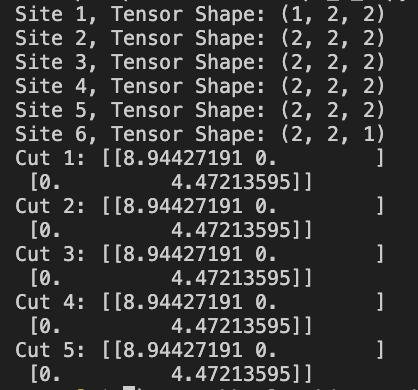
\includegraphics[width=\textwidth]{schmidt2.png}
\caption{Schmidt values across all cuts}
\end{figure}
% Inline Python code in the document
\begin{lstlisting}[language=Python]
import numpy as np
from p5_5 import truncate_svd

# Define MPS matrices for a chain
L = 6  # Number of sites
mps_tensors = []

# # Initial tensor setup
# A_1_up = np.array([1, 1]) / np.sqrt(2)
# A_1_down = np.array([1, -1]) / np.sqrt(2)
# mps_tensors.append(np.stack((A_1_up, A_1_down), axis=0).reshape(1, 2, 2))  # First tensor

# initial tensor setup for second part
A_1_up = np.array([1, 2])
A_1_down = np.array([2, -1])
mps_tensors.append(np.stack((A_1_up, A_1_down), axis=0).reshape(1, 2, 2))  # First tensor

# Middle tensors
for site in range(1, L-1):
    A_ell_up = np.array([[1, 1], [0, 0]]) / np.sqrt(2)
    A_ell_down = np.array([[0, 0], [1, -1]]) / np.sqrt(2)
    mps_tensors.append(np.stack((A_ell_up, A_ell_down), axis=0))

# # Last tensor
# A_L_up = np.array([1, 0])
# A_L_down = np.array([0, 1])
# mps_tensors.append(np.stack((A_L_up, A_L_down), axis=0).reshape(2, 2, 1))  # Last tensor

# last tensor for second part
A_L_up = np.array([1, 3])
A_L_down = np.array([3, 1])
mps_tensors.append(np.stack((A_L_up, A_L_down), axis=0).reshape(2, 2, 1))  # Last tensor


# Display tensor shapes
for idx, tensor in enumerate(mps_tensors):
    print(f"Site {idx+1}, Tensor Shape: {tensor.shape}")

# Calculate Schmidt values at each cut
for cut in range(1, L):
    # Contract tensors to the left of the cut
    left_state = mps_tensors[0].reshape(-1, 2)  # Start with the first tensor reshaped for matrix multiplication
    # first make a loop from 1 to cut - 1
    for i in range(1, cut):
        left_state = np.einsum('ab,bcd->acd', left_state, mps_tensors[i])
        left_state = left_state.reshape(-1, mps_tensors[i].shape[2])  # Ensure correct shape

    # Contract tensors to the right of the cut
    right_state = mps_tensors[cut].reshape(2, -1)  # Start with the tensor at the cut
    # now make a lope from cut+1 to L-1
    for j in range(cut + 1, L):
        right_state = np.einsum('abc,ad->cbd', mps_tensors[j], right_state)
        right_state = right_state.reshape(mps_tensors[j].shape[0], -1)  # Ensure correct shape

    # Compute the singular values directly from reshaped left and right states
    schmidt_matrix = np.dot(left_state, right_state)
    u, s, vt = truncate_svd(schmidt_matrix, 2)  # Adjust the truncation
    print(f"Cut {cut}: {s}")
\end{lstlisting}
\newpage
Now try bringing this MPS to the canonical form using the procedure described in the text. Start from the left end and move rightwards, performing appropriate SVDs on two-site blocks making all matrices to the left satisfy the left-canonical conditions. After reaching the right end, you will obtain the canonical form with the orthogonality center between $L-1$ and $L$. Now by moving leftwards performing appropriate SVDs, you can move the orthognality center to any location along the chain. As you do so, you can read off the true Schmidt values for the whole wavefunction at each cut and check against the results of the brute-force calculation in the previous paragraph. This procedure will be used extensively in Assignment 4, so make sure you get it well-tested here getting all the back-and-forth "reshapings" and groupings right.

Note that the cost of running this procedure is linear in $L$, so doubling the system size will take just two times longer (and not exponentially longer as in the brute-force approach).

\section*{References}
[1] Schollwöck, Ulrich. "The density-matrix renormalization group in the age of matrix product states." Annals of Physics 326, no. 1 (2011): 96-192.


\end{document}